\documentclass[twoside]{book}

% Packages required by doxygen
\usepackage{fixltx2e}
\usepackage{calc}
\usepackage{doxygen}
\usepackage{graphicx}
\usepackage[utf8]{inputenc}
\usepackage{makeidx}
\usepackage{multicol}
\usepackage{multirow}
\PassOptionsToPackage{warn}{textcomp}
\usepackage{textcomp}
\usepackage[nointegrals]{wasysym}
\usepackage[table]{xcolor}

% Font selection
\usepackage[T1]{fontenc}
\usepackage{mathptmx}
\usepackage[scaled=.90]{helvet}
\usepackage{courier}
\usepackage{amssymb}
\usepackage{sectsty}
\renewcommand{\familydefault}{\sfdefault}
\allsectionsfont{%
  \fontseries{bc}\selectfont%
  \color{darkgray}%
}
\renewcommand{\DoxyLabelFont}{%
  \fontseries{bc}\selectfont%
  \color{darkgray}%
}
\newcommand{\+}{\discretionary{\mbox{\scriptsize$\hookleftarrow$}}{}{}}

% Page & text layout
\usepackage{geometry}
\geometry{%
  a4paper,%
  top=2.5cm,%
  bottom=2.5cm,%
  left=2.5cm,%
  right=2.5cm%
}
\tolerance=750
\hfuzz=15pt
\hbadness=750
\setlength{\emergencystretch}{15pt}
\setlength{\parindent}{0cm}
\setlength{\parskip}{0.2cm}
\makeatletter
\renewcommand{\paragraph}{%
  \@startsection{paragraph}{4}{0ex}{-1.0ex}{1.0ex}{%
    \normalfont\normalsize\bfseries\SS@parafont%
  }%
}
\renewcommand{\subparagraph}{%
  \@startsection{subparagraph}{5}{0ex}{-1.0ex}{1.0ex}{%
    \normalfont\normalsize\bfseries\SS@subparafont%
  }%
}
\makeatother

% Headers & footers
\usepackage{fancyhdr}
\pagestyle{fancyplain}
\fancyhead[LE]{\fancyplain{}{\bfseries\thepage}}
\fancyhead[CE]{\fancyplain{}{}}
\fancyhead[RE]{\fancyplain{}{\bfseries\leftmark}}
\fancyhead[LO]{\fancyplain{}{\bfseries\rightmark}}
\fancyhead[CO]{\fancyplain{}{}}
\fancyhead[RO]{\fancyplain{}{\bfseries\thepage}}
\fancyfoot[LE]{\fancyplain{}{}}
\fancyfoot[CE]{\fancyplain{}{}}
\fancyfoot[RE]{\fancyplain{}{\bfseries\scriptsize Generated on Fri Feb 27 2015 05\+:03\+:48 for Chess by Doxygen }}
\fancyfoot[LO]{\fancyplain{}{\bfseries\scriptsize Generated on Fri Feb 27 2015 05\+:03\+:48 for Chess by Doxygen }}
\fancyfoot[CO]{\fancyplain{}{}}
\fancyfoot[RO]{\fancyplain{}{}}
\renewcommand{\footrulewidth}{0.4pt}
\renewcommand{\chaptermark}[1]{%
  \markboth{#1}{}%
}
\renewcommand{\sectionmark}[1]{%
  \markright{\thesection\ #1}%
}

% Indices & bibliography
\usepackage{natbib}
\usepackage[titles]{tocloft}
\setcounter{tocdepth}{3}
\setcounter{secnumdepth}{5}
\makeindex

% Hyperlinks (required, but should be loaded last)
\usepackage{ifpdf}
\ifpdf
  \usepackage[pdftex,pagebackref=true]{hyperref}
\else
  \usepackage[ps2pdf,pagebackref=true]{hyperref}
\fi
\hypersetup{%
  colorlinks=true,%
  linkcolor=blue,%
  citecolor=blue,%
  unicode%
}

% Custom commands
\newcommand{\clearemptydoublepage}{%
  \newpage{\pagestyle{empty}\cleardoublepage}%
}


%===== C O N T E N T S =====

\begin{document}

% Titlepage & ToC
\hypersetup{pageanchor=false,
             bookmarks=true,
             bookmarksnumbered=true,
             pdfencoding=unicode
            }
\pagenumbering{roman}
\begin{titlepage}
\vspace*{7cm}
\begin{center}%
{\Large Chess \\[1ex]\large 1.\+0.\+1 }\\
\vspace*{1cm}
{\large Generated by Doxygen 1.8.8}\\
\vspace*{0.5cm}
{\small Fri Feb 27 2015 05:03:48}\\
\end{center}
\end{titlepage}
\clearemptydoublepage
\tableofcontents
\clearemptydoublepage
\pagenumbering{arabic}
\hypersetup{pageanchor=true}

%--- Begin generated contents ---
\chapter{Hierarchical Index}
\section{Class Hierarchy}
This inheritance list is sorted roughly, but not completely, alphabetically\+:\begin{DoxyCompactList}
\item \contentsline{section}{models.\+Chess}{\pageref{classmodels_1_1_chess}}{}
\item \contentsline{section}{models.\+Chess\+Board}{\pageref{classmodels_1_1_chess_board}}{}
\item \contentsline{section}{chess\+Pieces.\+Chess\+Piece}{\pageref{classchess_pieces_1_1_chess_piece}}{}
\begin{DoxyCompactList}
\item \contentsline{section}{chess\+Pieces.\+Bishop}{\pageref{classchess_pieces_1_1_bishop}}{}
\item \contentsline{section}{chess\+Pieces.\+Empty}{\pageref{classchess_pieces_1_1_empty}}{}
\item \contentsline{section}{chess\+Pieces.\+King}{\pageref{classchess_pieces_1_1_king}}{}
\item \contentsline{section}{chess\+Pieces.\+Knight}{\pageref{classchess_pieces_1_1_knight}}{}
\item \contentsline{section}{chess\+Pieces.\+Pawn}{\pageref{classchess_pieces_1_1_pawn}}{}
\item \contentsline{section}{chess\+Pieces.\+Queen}{\pageref{classchess_pieces_1_1_queen}}{}
\item \contentsline{section}{chess\+Pieces.\+Rook}{\pageref{classchess_pieces_1_1_rook}}{}
\end{DoxyCompactList}
\item \contentsline{section}{models.\+Position}{\pageref{classmodels_1_1_position}}{}
\item \contentsline{section}{models.\+Record}{\pageref{classmodels_1_1_record}}{}
\end{DoxyCompactList}

\chapter{Class Index}
\section{Class List}
Here are the classes, structs, unions and interfaces with brief descriptions\+:\begin{DoxyCompactList}
\item\contentsline{section}{\hyperlink{classmodel_chess_pieces_1_1_bishop}{model\+Chess\+Pieces.\+Bishop} }{\pageref{classmodel_chess_pieces_1_1_bishop}}{}
\item\contentsline{section}{\hyperlink{classcontroller_1_1_chess}{controller.\+Chess} }{\pageref{classcontroller_1_1_chess}}{}
\item\contentsline{section}{\hyperlink{classmodel_core_1_1_chess_board}{model\+Core.\+Chess\+Board} }{\pageref{classmodel_core_1_1_chess_board}}{}
\item\contentsline{section}{\hyperlink{classmodel_chess_pieces_1_1_chess_piece}{model\+Chess\+Pieces.\+Chess\+Piece} }{\pageref{classmodel_chess_pieces_1_1_chess_piece}}{}
\item\contentsline{section}{\hyperlink{classmodel_chess_pieces_1_1_empress}{model\+Chess\+Pieces.\+Empress} }{\pageref{classmodel_chess_pieces_1_1_empress}}{}
\item\contentsline{section}{\hyperlink{classmodel_chess_pieces_1_1_empty}{model\+Chess\+Pieces.\+Empty} }{\pageref{classmodel_chess_pieces_1_1_empty}}{}
\item\contentsline{section}{\hyperlink{classviews_1_1_g_u_i}{views.\+G\+U\+I} }{\pageref{classviews_1_1_g_u_i}}{}
\item\contentsline{section}{\hyperlink{classmodel_chess_pieces_1_1_king}{model\+Chess\+Pieces.\+King} }{\pageref{classmodel_chess_pieces_1_1_king}}{}
\item\contentsline{section}{\hyperlink{classmodel_chess_pieces_1_1_knight}{model\+Chess\+Pieces.\+Knight} }{\pageref{classmodel_chess_pieces_1_1_knight}}{}
\item\contentsline{section}{\hyperlink{class_main}{Main} }{\pageref{class_main}}{}
\item\contentsline{section}{\hyperlink{classcontroller_1_1_menu_listener}{controller.\+Menu\+Listener} }{\pageref{classcontroller_1_1_menu_listener}}{}
\item\contentsline{section}{\hyperlink{classmodel_chess_pieces_1_1_pawn}{model\+Chess\+Pieces.\+Pawn} }{\pageref{classmodel_chess_pieces_1_1_pawn}}{}
\item\contentsline{section}{\hyperlink{classcontroller_1_1_piece_listener}{controller.\+Piece\+Listener} }{\pageref{classcontroller_1_1_piece_listener}}{}
\item\contentsline{section}{\hyperlink{classmodel_core_1_1_position}{model\+Core.\+Position} }{\pageref{classmodel_core_1_1_position}}{}
\item\contentsline{section}{\hyperlink{classmodel_chess_pieces_1_1_princess}{model\+Chess\+Pieces.\+Princess} }{\pageref{classmodel_chess_pieces_1_1_princess}}{}
\item\contentsline{section}{\hyperlink{classmodel_chess_pieces_1_1_queen}{model\+Chess\+Pieces.\+Queen} }{\pageref{classmodel_chess_pieces_1_1_queen}}{}
\item\contentsline{section}{\hyperlink{classmodel_core_1_1_record}{model\+Core.\+Record} }{\pageref{classmodel_core_1_1_record}}{}
\item\contentsline{section}{\hyperlink{classmodel_chess_pieces_1_1_rook}{model\+Chess\+Pieces.\+Rook} }{\pageref{classmodel_chess_pieces_1_1_rook}}{}
\end{DoxyCompactList}

\chapter{Class Documentation}
\hypertarget{classmodel_chess_pieces_1_1_bishop}{\section{model\+Chess\+Pieces.\+Bishop Class Reference}
\label{classmodel_chess_pieces_1_1_bishop}\index{model\+Chess\+Pieces.\+Bishop@{model\+Chess\+Pieces.\+Bishop}}
}
Inheritance diagram for model\+Chess\+Pieces.\+Bishop\+:\begin{figure}[H]
\begin{center}
\leavevmode
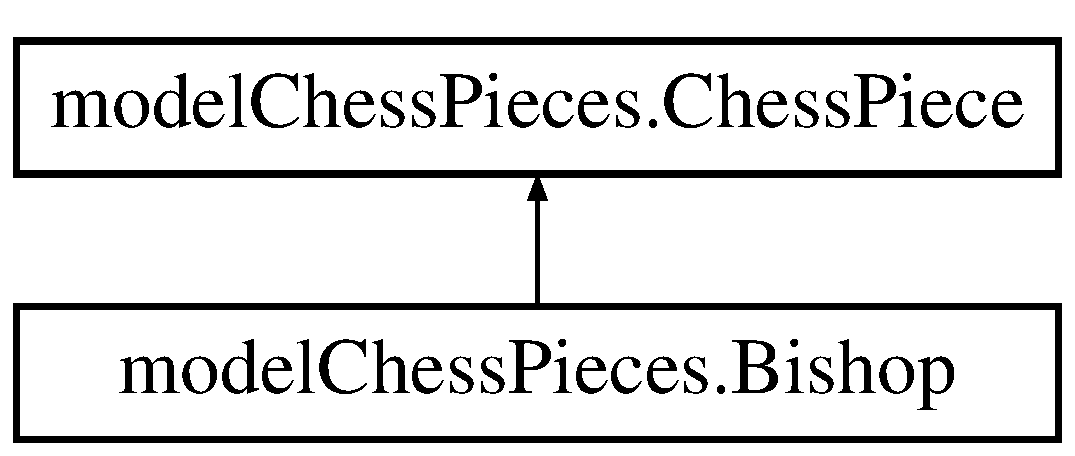
\includegraphics[height=2.000000cm]{classmodel_chess_pieces_1_1_bishop}
\end{center}
\end{figure}
\subsection*{Public Member Functions}
\begin{DoxyCompactItemize}
\item 
\hyperlink{classmodel_chess_pieces_1_1_bishop_ae2d6a71368f3304f8191acdf20949dc0}{Bishop} (String \hyperlink{classmodel_chess_pieces_1_1_chess_piece_a195487ca88c197af7c1604247be31db2}{type}, int \hyperlink{classmodel_chess_pieces_1_1_chess_piece_a979e63b99128333883acedc38d25dc87}{number})
\item 
\hyperlink{classmodel_chess_pieces_1_1_bishop_a224d00fc7396150863db9df71428a63c}{Bishop} (String \hyperlink{classmodel_chess_pieces_1_1_chess_piece_a195487ca88c197af7c1604247be31db2}{type}, \hyperlink{classmodel_core_1_1_position}{Position} \hyperlink{classmodel_chess_pieces_1_1_chess_piece_a3d4362d5b28f6edb14161196d9c6807d}{position}, int \hyperlink{classmodel_chess_pieces_1_1_chess_piece_a979e63b99128333883acedc38d25dc87}{number})
\item 
void \hyperlink{classmodel_chess_pieces_1_1_bishop_a55852b1b208028a1f87fbe46a1bf9337}{getpossible\+Next\+Positions} (\hyperlink{classmodel_core_1_1_chess_board}{Chess\+Board} chess\+Board)
\end{DoxyCompactItemize}
\subsection*{Additional Inherited Members}


\subsection{Detailed Description}
This is the class for bishop \begin{DoxyAuthor}{Author}
haoranyu 
\end{DoxyAuthor}
\begin{DoxySince}{Since}
2015-\/02-\/13 01\+:19\+:13 
\end{DoxySince}
\begin{DoxyVersion}{Version}
1.\+0 
\end{DoxyVersion}


\subsection{Constructor \& Destructor Documentation}
\hypertarget{classmodel_chess_pieces_1_1_bishop_ae2d6a71368f3304f8191acdf20949dc0}{\index{model\+Chess\+Pieces\+::\+Bishop@{model\+Chess\+Pieces\+::\+Bishop}!Bishop@{Bishop}}
\index{Bishop@{Bishop}!model\+Chess\+Pieces\+::\+Bishop@{model\+Chess\+Pieces\+::\+Bishop}}
\subsubsection[{Bishop}]{\setlength{\rightskip}{0pt plus 5cm}model\+Chess\+Pieces.\+Bishop.\+Bishop (
\begin{DoxyParamCaption}
\item[{String}]{type, }
\item[{int}]{number}
\end{DoxyParamCaption}
)}}\label{classmodel_chess_pieces_1_1_bishop_ae2d6a71368f3304f8191acdf20949dc0}
Constructor for default \hyperlink{classmodel_chess_pieces_1_1_bishop}{Bishop}


\begin{DoxyParams}{Parameters}
{\em type} & the color or null \\
\hline
{\em number} & the numbering of bishop \\
\hline
\end{DoxyParams}
\hypertarget{classmodel_chess_pieces_1_1_bishop_a224d00fc7396150863db9df71428a63c}{\index{model\+Chess\+Pieces\+::\+Bishop@{model\+Chess\+Pieces\+::\+Bishop}!Bishop@{Bishop}}
\index{Bishop@{Bishop}!model\+Chess\+Pieces\+::\+Bishop@{model\+Chess\+Pieces\+::\+Bishop}}
\subsubsection[{Bishop}]{\setlength{\rightskip}{0pt plus 5cm}model\+Chess\+Pieces.\+Bishop.\+Bishop (
\begin{DoxyParamCaption}
\item[{String}]{type, }
\item[{{\bf Position}}]{position, }
\item[{int}]{number}
\end{DoxyParamCaption}
)}}\label{classmodel_chess_pieces_1_1_bishop_a224d00fc7396150863db9df71428a63c}
Constructor for \hyperlink{classmodel_chess_pieces_1_1_bishop}{Bishop} with specified position


\begin{DoxyParams}{Parameters}
{\em type} & the color or null \\
\hline
{\em position} & the position of this bishop \\
\hline
{\em number} & the numbering of bishop \\
\hline
\end{DoxyParams}


\subsection{Member Function Documentation}
\hypertarget{classmodel_chess_pieces_1_1_bishop_a55852b1b208028a1f87fbe46a1bf9337}{\index{model\+Chess\+Pieces\+::\+Bishop@{model\+Chess\+Pieces\+::\+Bishop}!getpossible\+Next\+Positions@{getpossible\+Next\+Positions}}
\index{getpossible\+Next\+Positions@{getpossible\+Next\+Positions}!model\+Chess\+Pieces\+::\+Bishop@{model\+Chess\+Pieces\+::\+Bishop}}
\subsubsection[{getpossible\+Next\+Positions}]{\setlength{\rightskip}{0pt plus 5cm}void model\+Chess\+Pieces.\+Bishop.\+getpossible\+Next\+Positions (
\begin{DoxyParamCaption}
\item[{{\bf Chess\+Board}}]{chess\+Board}
\end{DoxyParamCaption}
)}}\label{classmodel_chess_pieces_1_1_bishop_a55852b1b208028a1f87fbe46a1bf9337}
Get all possible position for the next step


\begin{DoxyParams}{Parameters}
{\em chess\+Board} & the chess board we are now on \\
\hline
\end{DoxyParams}


The documentation for this class was generated from the following file\+:\begin{DoxyCompactItemize}
\item 
src/model\+Chess\+Pieces/Bishop.\+java\end{DoxyCompactItemize}

\hypertarget{classmodel_core_1_1_chess}{\section{model\+Core.\+Chess Class Reference}
\label{classmodel_core_1_1_chess}\index{model\+Core.\+Chess@{model\+Core.\+Chess}}
}
\subsection*{Static Public Member Functions}
\begin{DoxyCompactItemize}
\item 
static void \hyperlink{classmodel_core_1_1_chess_ad1b2d5c67a2d07367f36542ba9233d0b}{main} (String\mbox{[}$\,$\mbox{]} args)
\end{DoxyCompactItemize}


\subsection{Detailed Description}
\begin{DoxyAuthor}{Author}
haoranyu 
\end{DoxyAuthor}


\subsection{Member Function Documentation}
\hypertarget{classmodel_core_1_1_chess_ad1b2d5c67a2d07367f36542ba9233d0b}{\index{model\+Core\+::\+Chess@{model\+Core\+::\+Chess}!main@{main}}
\index{main@{main}!model\+Core\+::\+Chess@{model\+Core\+::\+Chess}}
\subsubsection[{main}]{\setlength{\rightskip}{0pt plus 5cm}static void model\+Core.\+Chess.\+main (
\begin{DoxyParamCaption}
\item[{String\mbox{[}$\,$\mbox{]}}]{args}
\end{DoxyParamCaption}
)\hspace{0.3cm}{\ttfamily [static]}}}\label{classmodel_core_1_1_chess_ad1b2d5c67a2d07367f36542ba9233d0b}

\begin{DoxyParams}{Parameters}
{\em args} & not specified \\
\hline
\end{DoxyParams}


The documentation for this class was generated from the following file\+:\begin{DoxyCompactItemize}
\item 
src/model\+Core/Chess.\+java\end{DoxyCompactItemize}

\hypertarget{classmodel_core_1_1_chess_board}{\section{model\+Core.\+Chess\+Board Class Reference}
\label{classmodel_core_1_1_chess_board}\index{model\+Core.\+Chess\+Board@{model\+Core.\+Chess\+Board}}
}
\subsection*{Public Member Functions}
\begin{DoxyCompactItemize}
\item 
\hyperlink{classmodel_core_1_1_chess_board_a50f1163eb1a59a7193668a8d1cf89435}{Chess\+Board} ()
\item 
\hyperlink{classmodel_core_1_1_chess_board_a74d33500fe30c1441989710578d9725d}{Chess\+Board} (\hyperlink{classmodel_core_1_1_chess_board}{Chess\+Board} chess\+Board)
\item 
\hyperlink{classmodel_chess_pieces_1_1_chess_piece}{Chess\+Piece} \hyperlink{classmodel_core_1_1_chess_board_ad700d180ac71927b8fd0e5c3e09ddd2b}{get\+Chess\+Piece\+In\+Position} (\hyperlink{classmodel_core_1_1_position}{Position} position)
\item 
void \hyperlink{classmodel_core_1_1_chess_board_af1a00d0d402bde8b8b5e5a23a96e6374}{set\+Chess\+Piece\+In\+Position} (\hyperlink{classmodel_core_1_1_position}{Position} position, \hyperlink{classmodel_chess_pieces_1_1_chess_piece}{Chess\+Piece} chess\+Piece)
\item 
void \hyperlink{classmodel_core_1_1_chess_board_a59800c1635a93d08909d34814bfffd20}{clear\+Position} (\hyperlink{classmodel_core_1_1_position}{Position} position)
\item 
boolean \hyperlink{classmodel_core_1_1_chess_board_abf420a5f1ea25fe7a8c6cdce3427c0af}{occupied} (\hyperlink{classmodel_core_1_1_position}{Position} position)
\item 
boolean \hyperlink{classmodel_core_1_1_chess_board_ab9216efa0fa5ce7794f813a500887647}{move} (\hyperlink{classmodel_chess_pieces_1_1_chess_piece}{Chess\+Piece} chess\+Piece, \hyperlink{classmodel_core_1_1_position}{Position} new\+Position)
\item 
boolean \hyperlink{classmodel_core_1_1_chess_board_aed20e0cd69a469134238b8ce28403e76}{self\+Checked} (\hyperlink{classmodel_chess_pieces_1_1_chess_piece}{Chess\+Piece} chess\+Piece)
\item 
boolean \hyperlink{classmodel_core_1_1_chess_board_a65d2495b5efc7db5a62e8af13ca0dda0}{check\+Other\+King} (\hyperlink{classmodel_chess_pieces_1_1_chess_piece}{Chess\+Piece} chess\+Piece)
\item 
boolean \hyperlink{classmodel_core_1_1_chess_board_a031a84fd458cb11464d0eadc6317b945}{is\+King\+Checked} (\hyperlink{classmodel_chess_pieces_1_1_chess_piece}{Chess\+Piece} king)
\item 
void \hyperlink{classmodel_core_1_1_chess_board_ad1bf119fff1c4af0b315c00ccec4c40b}{revert\+Move} ()
\item 
void \hyperlink{classmodel_core_1_1_chess_board_af36430e89b73d56b322509621d8b27ee}{add\+Record} (\hyperlink{classmodel_core_1_1_position}{Position} from\+Position, \hyperlink{classmodel_chess_pieces_1_1_chess_piece}{Chess\+Piece} from\+Chess\+Piece, \hyperlink{classmodel_core_1_1_position}{Position} to\+Position, \hyperlink{classmodel_chess_pieces_1_1_chess_piece}{Chess\+Piece} to\+Chess\+Piece)
\item 
Array\+List$<$ \hyperlink{classmodel_core_1_1_position}{Position} $>$ \hyperlink{classmodel_core_1_1_chess_board_a9580196da2802e440d64b5d6f8d50bf1}{all\+Possible\+Positions\+Of} (String color)
\item 
\hyperlink{classmodel_core_1_1_record}{Record} \hyperlink{classmodel_core_1_1_chess_board_ae899ac8bc62aaf23e4724870932ac6bf}{last\+Record} ()
\item 
String \hyperlink{classmodel_core_1_1_chess_board_a34e37f076c55fdc46d66ac2dc0280267}{get\+Win} ()
\item 
void \hyperlink{classmodel_core_1_1_chess_board_a504f3ee56db184a7e2d8a0aa0b4da1a5}{set\+Win} (String win)
\end{DoxyCompactItemize}
\subsection*{Public Attributes}
\begin{DoxyCompactItemize}
\item 
int \hyperlink{classmodel_core_1_1_chess_board_a97b8b44a011e141557812f801be59fb3}{row}
\item 
int \hyperlink{classmodel_core_1_1_chess_board_ad7110bd9ee10396094cb5a58406bd04e}{col}
\item 
\hyperlink{classmodel_chess_pieces_1_1_king}{King} \hyperlink{classmodel_core_1_1_chess_board_ac35268604f4e0b6c5b0b1a454f71f6b6}{white\+King}
\item 
\hyperlink{classmodel_chess_pieces_1_1_king}{King} \hyperlink{classmodel_core_1_1_chess_board_a4a811ce68180a71f5fea55095c3ef0f5}{black\+King}
\end{DoxyCompactItemize}


\subsection{Detailed Description}
\begin{DoxyAuthor}{Author}
haoranyu 
\end{DoxyAuthor}
\begin{DoxySince}{Since}
2015-\/02-\/16 03\+:56\+:14 
\end{DoxySince}
\begin{DoxyVersion}{Version}
1.\+1 
\end{DoxyVersion}


\subsection{Constructor \& Destructor Documentation}
\hypertarget{classmodel_core_1_1_chess_board_a50f1163eb1a59a7193668a8d1cf89435}{\index{model\+Core\+::\+Chess\+Board@{model\+Core\+::\+Chess\+Board}!Chess\+Board@{Chess\+Board}}
\index{Chess\+Board@{Chess\+Board}!model\+Core\+::\+Chess\+Board@{model\+Core\+::\+Chess\+Board}}
\subsubsection[{Chess\+Board}]{\setlength{\rightskip}{0pt plus 5cm}model\+Core.\+Chess\+Board.\+Chess\+Board (
\begin{DoxyParamCaption}
{}
\end{DoxyParamCaption}
)}}\label{classmodel_core_1_1_chess_board_a50f1163eb1a59a7193668a8d1cf89435}
Constructor for a new chess\+Board with chess pieces defined \hypertarget{classmodel_core_1_1_chess_board_a74d33500fe30c1441989710578d9725d}{\index{model\+Core\+::\+Chess\+Board@{model\+Core\+::\+Chess\+Board}!Chess\+Board@{Chess\+Board}}
\index{Chess\+Board@{Chess\+Board}!model\+Core\+::\+Chess\+Board@{model\+Core\+::\+Chess\+Board}}
\subsubsection[{Chess\+Board}]{\setlength{\rightskip}{0pt plus 5cm}model\+Core.\+Chess\+Board.\+Chess\+Board (
\begin{DoxyParamCaption}
\item[{{\bf Chess\+Board}}]{chess\+Board}
\end{DoxyParamCaption}
)}}\label{classmodel_core_1_1_chess_board_a74d33500fe30c1441989710578d9725d}
Copy Constructor 

\subsection{Member Function Documentation}
\hypertarget{classmodel_core_1_1_chess_board_af36430e89b73d56b322509621d8b27ee}{\index{model\+Core\+::\+Chess\+Board@{model\+Core\+::\+Chess\+Board}!add\+Record@{add\+Record}}
\index{add\+Record@{add\+Record}!model\+Core\+::\+Chess\+Board@{model\+Core\+::\+Chess\+Board}}
\subsubsection[{add\+Record}]{\setlength{\rightskip}{0pt plus 5cm}void model\+Core.\+Chess\+Board.\+add\+Record (
\begin{DoxyParamCaption}
\item[{{\bf Position}}]{from\+Position, }
\item[{{\bf Chess\+Piece}}]{from\+Chess\+Piece, }
\item[{{\bf Position}}]{to\+Position, }
\item[{{\bf Chess\+Piece}}]{to\+Chess\+Piece}
\end{DoxyParamCaption}
)}}\label{classmodel_core_1_1_chess_board_af36430e89b73d56b322509621d8b27ee}
A function for adding a new record 
\begin{DoxyParams}{Parameters}
{\em from\+Position} & \\
\hline
{\em from\+Chess\+Piece} & \\
\hline
{\em to\+Position} & \\
\hline
{\em to\+Chess\+Piece} & \\
\hline
\end{DoxyParams}
\hypertarget{classmodel_core_1_1_chess_board_a9580196da2802e440d64b5d6f8d50bf1}{\index{model\+Core\+::\+Chess\+Board@{model\+Core\+::\+Chess\+Board}!all\+Possible\+Positions\+Of@{all\+Possible\+Positions\+Of}}
\index{all\+Possible\+Positions\+Of@{all\+Possible\+Positions\+Of}!model\+Core\+::\+Chess\+Board@{model\+Core\+::\+Chess\+Board}}
\subsubsection[{all\+Possible\+Positions\+Of}]{\setlength{\rightskip}{0pt plus 5cm}Array\+List$<${\bf Position}$>$ model\+Core.\+Chess\+Board.\+all\+Possible\+Positions\+Of (
\begin{DoxyParamCaption}
\item[{String}]{color}
\end{DoxyParamCaption}
)}}\label{classmodel_core_1_1_chess_board_a9580196da2802e440d64b5d6f8d50bf1}
Find all possible positions for the chess pieces of player of C\+O\+L\+O\+R to move 
\begin{DoxyParams}{Parameters}
{\em color} & the player color \\
\hline
\end{DoxyParams}
\begin{DoxyReturn}{Returns}
all possible positions for the chess pieces of player of C\+O\+L\+O\+R to move 
\end{DoxyReturn}
\hypertarget{classmodel_core_1_1_chess_board_a65d2495b5efc7db5a62e8af13ca0dda0}{\index{model\+Core\+::\+Chess\+Board@{model\+Core\+::\+Chess\+Board}!check\+Other\+King@{check\+Other\+King}}
\index{check\+Other\+King@{check\+Other\+King}!model\+Core\+::\+Chess\+Board@{model\+Core\+::\+Chess\+Board}}
\subsubsection[{check\+Other\+King}]{\setlength{\rightskip}{0pt plus 5cm}boolean model\+Core.\+Chess\+Board.\+check\+Other\+King (
\begin{DoxyParamCaption}
\item[{{\bf Chess\+Piece}}]{chess\+Piece}
\end{DoxyParamCaption}
)}}\label{classmodel_core_1_1_chess_board_a65d2495b5efc7db5a62e8af13ca0dda0}
See whether the chess piece is now checking the other king and should win the game


\begin{DoxyParams}{Parameters}
{\em chess\+Piece} & the chess\+Piece it is now moving \\
\hline
\end{DoxyParams}
\begin{DoxyReturn}{Returns}
True if there king of others is under check-\/mate 
\end{DoxyReturn}
\hypertarget{classmodel_core_1_1_chess_board_a59800c1635a93d08909d34814bfffd20}{\index{model\+Core\+::\+Chess\+Board@{model\+Core\+::\+Chess\+Board}!clear\+Position@{clear\+Position}}
\index{clear\+Position@{clear\+Position}!model\+Core\+::\+Chess\+Board@{model\+Core\+::\+Chess\+Board}}
\subsubsection[{clear\+Position}]{\setlength{\rightskip}{0pt plus 5cm}void model\+Core.\+Chess\+Board.\+clear\+Position (
\begin{DoxyParamCaption}
\item[{{\bf Position}}]{position}
\end{DoxyParamCaption}
)}}\label{classmodel_core_1_1_chess_board_a59800c1635a93d08909d34814bfffd20}
Make the cell of position null


\begin{DoxyParams}{Parameters}
{\em position} & The position we want to clear \\
\hline
\end{DoxyParams}
\hypertarget{classmodel_core_1_1_chess_board_ad700d180ac71927b8fd0e5c3e09ddd2b}{\index{model\+Core\+::\+Chess\+Board@{model\+Core\+::\+Chess\+Board}!get\+Chess\+Piece\+In\+Position@{get\+Chess\+Piece\+In\+Position}}
\index{get\+Chess\+Piece\+In\+Position@{get\+Chess\+Piece\+In\+Position}!model\+Core\+::\+Chess\+Board@{model\+Core\+::\+Chess\+Board}}
\subsubsection[{get\+Chess\+Piece\+In\+Position}]{\setlength{\rightskip}{0pt plus 5cm}{\bf Chess\+Piece} model\+Core.\+Chess\+Board.\+get\+Chess\+Piece\+In\+Position (
\begin{DoxyParamCaption}
\item[{{\bf Position}}]{position}
\end{DoxyParamCaption}
)}}\label{classmodel_core_1_1_chess_board_ad700d180ac71927b8fd0e5c3e09ddd2b}
Get the chess\+Piece in the position


\begin{DoxyParams}{Parameters}
{\em position} & The position we see into \\
\hline
\end{DoxyParams}
\begin{DoxyReturn}{Returns}
chess\+Piece Return the chess piece in this position $\vert$ Null if not valid 
\end{DoxyReturn}
\hypertarget{classmodel_core_1_1_chess_board_a34e37f076c55fdc46d66ac2dc0280267}{\index{model\+Core\+::\+Chess\+Board@{model\+Core\+::\+Chess\+Board}!get\+Win@{get\+Win}}
\index{get\+Win@{get\+Win}!model\+Core\+::\+Chess\+Board@{model\+Core\+::\+Chess\+Board}}
\subsubsection[{get\+Win}]{\setlength{\rightskip}{0pt plus 5cm}String model\+Core.\+Chess\+Board.\+get\+Win (
\begin{DoxyParamCaption}
{}
\end{DoxyParamCaption}
)}}\label{classmodel_core_1_1_chess_board_a34e37f076c55fdc46d66ac2dc0280267}
\begin{DoxyReturn}{Returns}
the win 
\end{DoxyReturn}
\hypertarget{classmodel_core_1_1_chess_board_a031a84fd458cb11464d0eadc6317b945}{\index{model\+Core\+::\+Chess\+Board@{model\+Core\+::\+Chess\+Board}!is\+King\+Checked@{is\+King\+Checked}}
\index{is\+King\+Checked@{is\+King\+Checked}!model\+Core\+::\+Chess\+Board@{model\+Core\+::\+Chess\+Board}}
\subsubsection[{is\+King\+Checked}]{\setlength{\rightskip}{0pt plus 5cm}boolean model\+Core.\+Chess\+Board.\+is\+King\+Checked (
\begin{DoxyParamCaption}
\item[{{\bf Chess\+Piece}}]{king}
\end{DoxyParamCaption}
)}}\label{classmodel_core_1_1_chess_board_a031a84fd458cb11464d0eadc6317b945}
Check whether a king is under check 
\begin{DoxyParams}{Parameters}
{\em king} & \\
\hline
\end{DoxyParams}
\begin{DoxyReturn}{Returns}

\end{DoxyReturn}
\hypertarget{classmodel_core_1_1_chess_board_ae899ac8bc62aaf23e4724870932ac6bf}{\index{model\+Core\+::\+Chess\+Board@{model\+Core\+::\+Chess\+Board}!last\+Record@{last\+Record}}
\index{last\+Record@{last\+Record}!model\+Core\+::\+Chess\+Board@{model\+Core\+::\+Chess\+Board}}
\subsubsection[{last\+Record}]{\setlength{\rightskip}{0pt plus 5cm}{\bf Record} model\+Core.\+Chess\+Board.\+last\+Record (
\begin{DoxyParamCaption}
{}
\end{DoxyParamCaption}
)}}\label{classmodel_core_1_1_chess_board_ae899ac8bc62aaf23e4724870932ac6bf}
\begin{DoxyReturn}{Returns}
the last pushed in record 
\end{DoxyReturn}
\hypertarget{classmodel_core_1_1_chess_board_ab9216efa0fa5ce7794f813a500887647}{\index{model\+Core\+::\+Chess\+Board@{model\+Core\+::\+Chess\+Board}!move@{move}}
\index{move@{move}!model\+Core\+::\+Chess\+Board@{model\+Core\+::\+Chess\+Board}}
\subsubsection[{move}]{\setlength{\rightskip}{0pt plus 5cm}boolean model\+Core.\+Chess\+Board.\+move (
\begin{DoxyParamCaption}
\item[{{\bf Chess\+Piece}}]{chess\+Piece, }
\item[{{\bf Position}}]{new\+Position}
\end{DoxyParamCaption}
)}}\label{classmodel_core_1_1_chess_board_ab9216efa0fa5ce7794f813a500887647}
The move function for a chess\+Piece to move


\begin{DoxyParams}{Parameters}
{\em chess\+Piece} & The chess\+Piece to move \\
\hline
{\em new\+Position} & The position we are moving to \\
\hline
\end{DoxyParams}
\begin{DoxyReturn}{Returns}
Return true if it is possible 
\end{DoxyReturn}
\hypertarget{classmodel_core_1_1_chess_board_abf420a5f1ea25fe7a8c6cdce3427c0af}{\index{model\+Core\+::\+Chess\+Board@{model\+Core\+::\+Chess\+Board}!occupied@{occupied}}
\index{occupied@{occupied}!model\+Core\+::\+Chess\+Board@{model\+Core\+::\+Chess\+Board}}
\subsubsection[{occupied}]{\setlength{\rightskip}{0pt plus 5cm}boolean model\+Core.\+Chess\+Board.\+occupied (
\begin{DoxyParamCaption}
\item[{{\bf Position}}]{position}
\end{DoxyParamCaption}
)}}\label{classmodel_core_1_1_chess_board_abf420a5f1ea25fe7a8c6cdce3427c0af}
Check if the position is occupied by any chess piece


\begin{DoxyParams}{Parameters}
{\em position} & The position we see into \\
\hline
\end{DoxyParams}
\begin{DoxyReturn}{Returns}
True if any chess piece in this position 
\end{DoxyReturn}
\hypertarget{classmodel_core_1_1_chess_board_ad1bf119fff1c4af0b315c00ccec4c40b}{\index{model\+Core\+::\+Chess\+Board@{model\+Core\+::\+Chess\+Board}!revert\+Move@{revert\+Move}}
\index{revert\+Move@{revert\+Move}!model\+Core\+::\+Chess\+Board@{model\+Core\+::\+Chess\+Board}}
\subsubsection[{revert\+Move}]{\setlength{\rightskip}{0pt plus 5cm}void model\+Core.\+Chess\+Board.\+revert\+Move (
\begin{DoxyParamCaption}
{}
\end{DoxyParamCaption}
)}}\label{classmodel_core_1_1_chess_board_ad1bf119fff1c4af0b315c00ccec4c40b}
Revert the last move \hypertarget{classmodel_core_1_1_chess_board_aed20e0cd69a469134238b8ce28403e76}{\index{model\+Core\+::\+Chess\+Board@{model\+Core\+::\+Chess\+Board}!self\+Checked@{self\+Checked}}
\index{self\+Checked@{self\+Checked}!model\+Core\+::\+Chess\+Board@{model\+Core\+::\+Chess\+Board}}
\subsubsection[{self\+Checked}]{\setlength{\rightskip}{0pt plus 5cm}boolean model\+Core.\+Chess\+Board.\+self\+Checked (
\begin{DoxyParamCaption}
\item[{{\bf Chess\+Piece}}]{chess\+Piece}
\end{DoxyParamCaption}
)}}\label{classmodel_core_1_1_chess_board_aed20e0cd69a469134238b8ce28403e76}
Judge whether 
\begin{DoxyParams}{Parameters}
{\em chess\+Piece} & \\
\hline
\end{DoxyParams}
\begin{DoxyReturn}{Returns}

\end{DoxyReturn}
\hypertarget{classmodel_core_1_1_chess_board_af1a00d0d402bde8b8b5e5a23a96e6374}{\index{model\+Core\+::\+Chess\+Board@{model\+Core\+::\+Chess\+Board}!set\+Chess\+Piece\+In\+Position@{set\+Chess\+Piece\+In\+Position}}
\index{set\+Chess\+Piece\+In\+Position@{set\+Chess\+Piece\+In\+Position}!model\+Core\+::\+Chess\+Board@{model\+Core\+::\+Chess\+Board}}
\subsubsection[{set\+Chess\+Piece\+In\+Position}]{\setlength{\rightskip}{0pt plus 5cm}void model\+Core.\+Chess\+Board.\+set\+Chess\+Piece\+In\+Position (
\begin{DoxyParamCaption}
\item[{{\bf Position}}]{position, }
\item[{{\bf Chess\+Piece}}]{chess\+Piece}
\end{DoxyParamCaption}
)}}\label{classmodel_core_1_1_chess_board_af1a00d0d402bde8b8b5e5a23a96e6374}
Set a chess\+Piece into the chess\+Board


\begin{DoxyParams}{Parameters}
{\em position} & The position we see into \\
\hline
{\em chess\+Piece} & The chess piece we want to put into the position \\
\hline
\end{DoxyParams}
\hypertarget{classmodel_core_1_1_chess_board_a504f3ee56db184a7e2d8a0aa0b4da1a5}{\index{model\+Core\+::\+Chess\+Board@{model\+Core\+::\+Chess\+Board}!set\+Win@{set\+Win}}
\index{set\+Win@{set\+Win}!model\+Core\+::\+Chess\+Board@{model\+Core\+::\+Chess\+Board}}
\subsubsection[{set\+Win}]{\setlength{\rightskip}{0pt plus 5cm}void model\+Core.\+Chess\+Board.\+set\+Win (
\begin{DoxyParamCaption}
\item[{String}]{win}
\end{DoxyParamCaption}
)}}\label{classmodel_core_1_1_chess_board_a504f3ee56db184a7e2d8a0aa0b4da1a5}

\begin{DoxyParams}{Parameters}
{\em win} & the win to set \\
\hline
\end{DoxyParams}


\subsection{Member Data Documentation}
\hypertarget{classmodel_core_1_1_chess_board_a4a811ce68180a71f5fea55095c3ef0f5}{\index{model\+Core\+::\+Chess\+Board@{model\+Core\+::\+Chess\+Board}!black\+King@{black\+King}}
\index{black\+King@{black\+King}!model\+Core\+::\+Chess\+Board@{model\+Core\+::\+Chess\+Board}}
\subsubsection[{black\+King}]{\setlength{\rightskip}{0pt plus 5cm}{\bf King} model\+Core.\+Chess\+Board.\+black\+King}}\label{classmodel_core_1_1_chess_board_a4a811ce68180a71f5fea55095c3ef0f5}
since king is unique we set it as a member of \hyperlink{classmodel_core_1_1_chess_board}{Chess\+Board} which is also easier to access \hypertarget{classmodel_core_1_1_chess_board_ad7110bd9ee10396094cb5a58406bd04e}{\index{model\+Core\+::\+Chess\+Board@{model\+Core\+::\+Chess\+Board}!col@{col}}
\index{col@{col}!model\+Core\+::\+Chess\+Board@{model\+Core\+::\+Chess\+Board}}
\subsubsection[{col}]{\setlength{\rightskip}{0pt plus 5cm}int model\+Core.\+Chess\+Board.\+col}}\label{classmodel_core_1_1_chess_board_ad7110bd9ee10396094cb5a58406bd04e}
how many columns for the chess board \hypertarget{classmodel_core_1_1_chess_board_a97b8b44a011e141557812f801be59fb3}{\index{model\+Core\+::\+Chess\+Board@{model\+Core\+::\+Chess\+Board}!row@{row}}
\index{row@{row}!model\+Core\+::\+Chess\+Board@{model\+Core\+::\+Chess\+Board}}
\subsubsection[{row}]{\setlength{\rightskip}{0pt plus 5cm}int model\+Core.\+Chess\+Board.\+row}}\label{classmodel_core_1_1_chess_board_a97b8b44a011e141557812f801be59fb3}
how many rows for the chess board \hypertarget{classmodel_core_1_1_chess_board_ac35268604f4e0b6c5b0b1a454f71f6b6}{\index{model\+Core\+::\+Chess\+Board@{model\+Core\+::\+Chess\+Board}!white\+King@{white\+King}}
\index{white\+King@{white\+King}!model\+Core\+::\+Chess\+Board@{model\+Core\+::\+Chess\+Board}}
\subsubsection[{white\+King}]{\setlength{\rightskip}{0pt plus 5cm}{\bf King} model\+Core.\+Chess\+Board.\+white\+King}}\label{classmodel_core_1_1_chess_board_ac35268604f4e0b6c5b0b1a454f71f6b6}
since king is unique we set it as a member of \hyperlink{classmodel_core_1_1_chess_board}{Chess\+Board} which is also easier to access 

The documentation for this class was generated from the following file\+:\begin{DoxyCompactItemize}
\item 
src/model\+Core/Chess\+Board.\+java\end{DoxyCompactItemize}

\hypertarget{classmodel_chess_pieces_1_1_chess_piece}{\section{model\+Chess\+Pieces.\+Chess\+Piece Class Reference}
\label{classmodel_chess_pieces_1_1_chess_piece}\index{model\+Chess\+Pieces.\+Chess\+Piece@{model\+Chess\+Pieces.\+Chess\+Piece}}
}
Inheritance diagram for model\+Chess\+Pieces.\+Chess\+Piece\+:\begin{figure}[H]
\begin{center}
\leavevmode
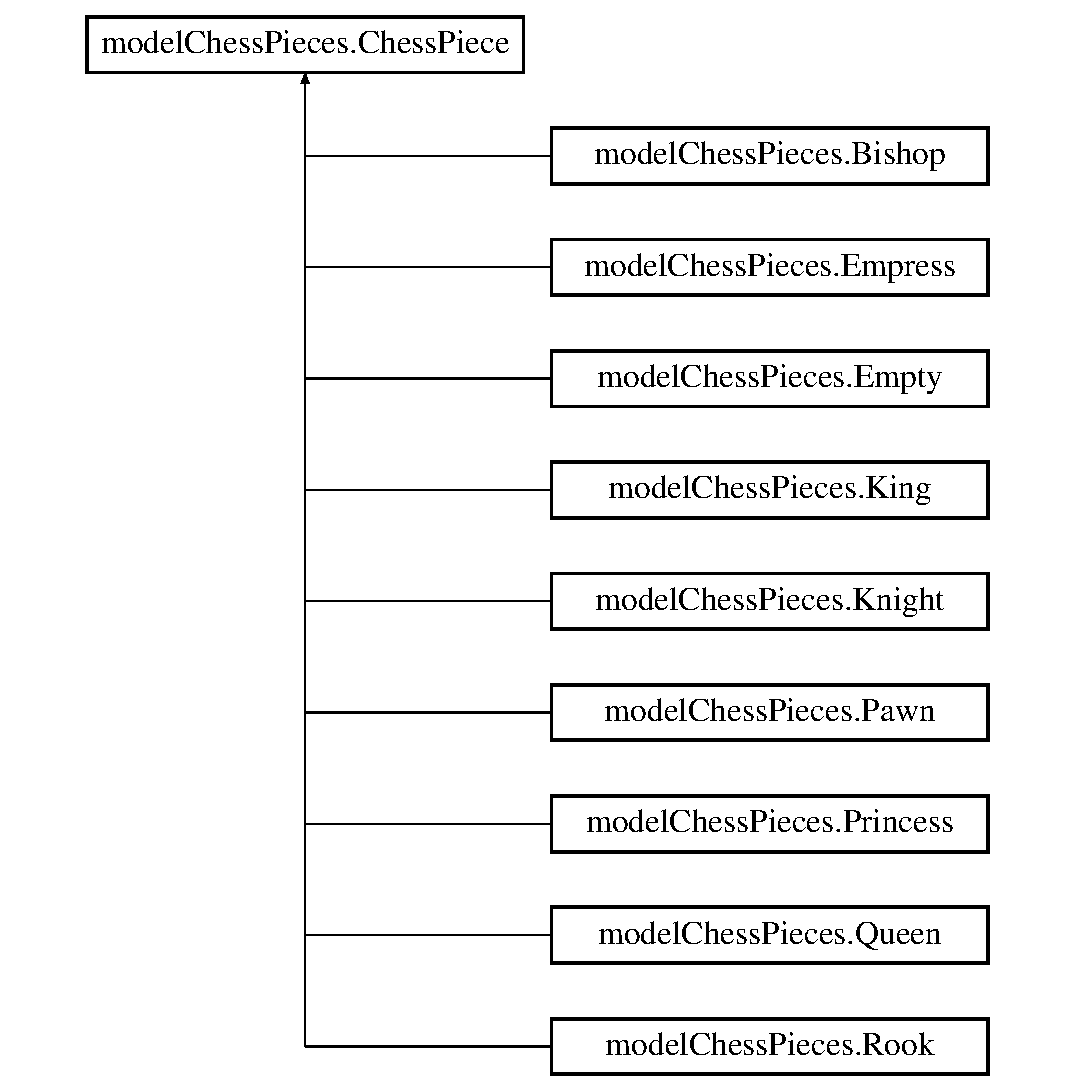
\includegraphics[height=10.000000cm]{classmodel_chess_pieces_1_1_chess_piece}
\end{center}
\end{figure}
\subsection*{Public Member Functions}
\begin{DoxyCompactItemize}
\item 
void \hyperlink{classmodel_chess_pieces_1_1_chess_piece_a70a2f0f1a29b9545fcad604df3ad89c2}{showpossible\+Next\+Positions} (\hyperlink{classmodel_core_1_1_chess_board}{Chess\+Board} chess\+Board)
\item 
abstract void \hyperlink{classmodel_chess_pieces_1_1_chess_piece_a920de36744a00c01fde87cb4a12e4dec}{getpossible\+Next\+Positions} (\hyperlink{classmodel_core_1_1_chess_board}{Chess\+Board} chess\+Board)
\item 
\hyperlink{classmodel_core_1_1_position}{Position} \hyperlink{classmodel_chess_pieces_1_1_chess_piece_a6e88271516d06a50162a36321d10ff0e}{get\+Position} ()
\item 
void \hyperlink{classmodel_chess_pieces_1_1_chess_piece_abdd69cca4ca429e531ab58297c0036c7}{set\+Position} (\hyperlink{classmodel_core_1_1_position}{Position} \hyperlink{classmodel_chess_pieces_1_1_chess_piece_a3d4362d5b28f6edb14161196d9c6807d}{position})
\item 
String \hyperlink{classmodel_chess_pieces_1_1_chess_piece_a09214c36497f15c4d85af11a8dd8bfed}{get\+Enemy\+Type} ()
\item 
String \hyperlink{classmodel_chess_pieces_1_1_chess_piece_a189d923d883085ce16d051c161c93e68}{get\+Type} ()
\item 
void \hyperlink{classmodel_chess_pieces_1_1_chess_piece_a7d2fa4377c4409371487f3e5afd5e100}{set\+Type} (String \hyperlink{classmodel_chess_pieces_1_1_chess_piece_a195487ca88c197af7c1604247be31db2}{type})
\item 
String \hyperlink{classmodel_chess_pieces_1_1_chess_piece_ac73d3ae34142cdbf7571a086ffb122c9}{get\+Name} ()
\item 
void \hyperlink{classmodel_chess_pieces_1_1_chess_piece_a86e3e4135360b5bdc7ce9f6bad817b99}{set\+Name} (String \hyperlink{classmodel_chess_pieces_1_1_chess_piece_a03d2fb76fbbff0dab72d00f2173a69ff}{name})
\item 
boolean \hyperlink{classmodel_chess_pieces_1_1_chess_piece_ad6b3bbf9101c70a29ad8087f9431b8ee}{is\+Moved} ()
\item 
void \hyperlink{classmodel_chess_pieces_1_1_chess_piece_a43b4de8cc87600ac934d85cb09c852a1}{set\+Moved} (boolean \hyperlink{classmodel_chess_pieces_1_1_chess_piece_a5bc0722badda5dc066b6a73476fc933c}{moved})
\end{DoxyCompactItemize}
\subsection*{Public Attributes}
\begin{DoxyCompactItemize}
\item 
Array\+List$<$ \hyperlink{classmodel_core_1_1_position}{Position} $>$ \hyperlink{classmodel_chess_pieces_1_1_chess_piece_aa477ac8d33b4e7c98eb6f4aec2390477}{possible\+Next\+Positions} = new Array\+List$<$$>$()
\end{DoxyCompactItemize}
\subsection*{Protected Member Functions}
\begin{DoxyCompactItemize}
\item 
boolean \hyperlink{classmodel_chess_pieces_1_1_chess_piece_a8045974b8d8f1e88722cd54b050774c5}{self\+Occupied} (\hyperlink{classmodel_core_1_1_chess_board}{Chess\+Board} chess\+Board, \hyperlink{classmodel_core_1_1_position}{Position} \hyperlink{classmodel_chess_pieces_1_1_chess_piece_a3d4362d5b28f6edb14161196d9c6807d}{position})
\item 
boolean \hyperlink{classmodel_chess_pieces_1_1_chess_piece_a247db1a354f7792b0a79b8128629a1c5}{add\+If\+Avaliable} (\hyperlink{classmodel_core_1_1_chess_board}{Chess\+Board} chess\+Board, \hyperlink{classmodel_core_1_1_position}{Position} \hyperlink{classmodel_chess_pieces_1_1_chess_piece_a3d4362d5b28f6edb14161196d9c6807d}{position})
\item 
void \hyperlink{classmodel_chess_pieces_1_1_chess_piece_a86900a063a4596d7445e8bd2af895445}{iterative\+Add\+Possible\+Position} (\hyperlink{classmodel_core_1_1_chess_board}{Chess\+Board} chess\+Board, \hyperlink{classmodel_core_1_1_position}{Position} start\+Position, int x\+Delta, int y\+Delta)
\end{DoxyCompactItemize}
\subsection*{Protected Attributes}
\begin{DoxyCompactItemize}
\item 
boolean \hyperlink{classmodel_chess_pieces_1_1_chess_piece_a5bc0722badda5dc066b6a73476fc933c}{moved}
\item 
String \hyperlink{classmodel_chess_pieces_1_1_chess_piece_a03d2fb76fbbff0dab72d00f2173a69ff}{name}
\item 
String \hyperlink{classmodel_chess_pieces_1_1_chess_piece_a195487ca88c197af7c1604247be31db2}{type}
\item 
int \hyperlink{classmodel_chess_pieces_1_1_chess_piece_a979e63b99128333883acedc38d25dc87}{number}
\item 
\hyperlink{classmodel_core_1_1_position}{Position} \hyperlink{classmodel_chess_pieces_1_1_chess_piece_a3d4362d5b28f6edb14161196d9c6807d}{position}
\end{DoxyCompactItemize}


\subsection{Detailed Description}
\begin{DoxyAuthor}{Author}
haoranyu 
\end{DoxyAuthor}
\begin{DoxySince}{Since}
2015-\/02-\/16 03\+:56\+:20 
\end{DoxySince}
\begin{DoxyVersion}{Version}
1.\+1 
\end{DoxyVersion}


\subsection{Member Function Documentation}
\hypertarget{classmodel_chess_pieces_1_1_chess_piece_a247db1a354f7792b0a79b8128629a1c5}{\index{model\+Chess\+Pieces\+::\+Chess\+Piece@{model\+Chess\+Pieces\+::\+Chess\+Piece}!add\+If\+Avaliable@{add\+If\+Avaliable}}
\index{add\+If\+Avaliable@{add\+If\+Avaliable}!model\+Chess\+Pieces\+::\+Chess\+Piece@{model\+Chess\+Pieces\+::\+Chess\+Piece}}
\subsubsection[{add\+If\+Avaliable}]{\setlength{\rightskip}{0pt plus 5cm}boolean model\+Chess\+Pieces.\+Chess\+Piece.\+add\+If\+Avaliable (
\begin{DoxyParamCaption}
\item[{{\bf Chess\+Board}}]{chess\+Board, }
\item[{{\bf Position}}]{position}
\end{DoxyParamCaption}
)\hspace{0.3cm}{\ttfamily [protected]}}}\label{classmodel_chess_pieces_1_1_chess_piece_a247db1a354f7792b0a79b8128629a1c5}
If the cell is valid A\+N\+D is not self-\/occupied A\+N\+D not duplicates, Then add to possible position


\begin{DoxyParams}{Parameters}
{\em chess\+Board} & The object of chess board \\
\hline
{\em position} & The position we see into \\
\hline
\end{DoxyParams}
\begin{DoxyReturn}{Returns}
Return true if the outer iteration should going on 
\end{DoxyReturn}
\hypertarget{classmodel_chess_pieces_1_1_chess_piece_a09214c36497f15c4d85af11a8dd8bfed}{\index{model\+Chess\+Pieces\+::\+Chess\+Piece@{model\+Chess\+Pieces\+::\+Chess\+Piece}!get\+Enemy\+Type@{get\+Enemy\+Type}}
\index{get\+Enemy\+Type@{get\+Enemy\+Type}!model\+Chess\+Pieces\+::\+Chess\+Piece@{model\+Chess\+Pieces\+::\+Chess\+Piece}}
\subsubsection[{get\+Enemy\+Type}]{\setlength{\rightskip}{0pt plus 5cm}String model\+Chess\+Pieces.\+Chess\+Piece.\+get\+Enemy\+Type (
\begin{DoxyParamCaption}
{}
\end{DoxyParamCaption}
)}}\label{classmodel_chess_pieces_1_1_chess_piece_a09214c36497f15c4d85af11a8dd8bfed}
\begin{DoxyReturn}{Returns}
the enemy type 
\end{DoxyReturn}
\hypertarget{classmodel_chess_pieces_1_1_chess_piece_ac73d3ae34142cdbf7571a086ffb122c9}{\index{model\+Chess\+Pieces\+::\+Chess\+Piece@{model\+Chess\+Pieces\+::\+Chess\+Piece}!get\+Name@{get\+Name}}
\index{get\+Name@{get\+Name}!model\+Chess\+Pieces\+::\+Chess\+Piece@{model\+Chess\+Pieces\+::\+Chess\+Piece}}
\subsubsection[{get\+Name}]{\setlength{\rightskip}{0pt plus 5cm}String model\+Chess\+Pieces.\+Chess\+Piece.\+get\+Name (
\begin{DoxyParamCaption}
{}
\end{DoxyParamCaption}
)}}\label{classmodel_chess_pieces_1_1_chess_piece_ac73d3ae34142cdbf7571a086ffb122c9}
\begin{DoxyReturn}{Returns}
the name 
\end{DoxyReturn}
\hypertarget{classmodel_chess_pieces_1_1_chess_piece_a6e88271516d06a50162a36321d10ff0e}{\index{model\+Chess\+Pieces\+::\+Chess\+Piece@{model\+Chess\+Pieces\+::\+Chess\+Piece}!get\+Position@{get\+Position}}
\index{get\+Position@{get\+Position}!model\+Chess\+Pieces\+::\+Chess\+Piece@{model\+Chess\+Pieces\+::\+Chess\+Piece}}
\subsubsection[{get\+Position}]{\setlength{\rightskip}{0pt plus 5cm}{\bf Position} model\+Chess\+Pieces.\+Chess\+Piece.\+get\+Position (
\begin{DoxyParamCaption}
{}
\end{DoxyParamCaption}
)}}\label{classmodel_chess_pieces_1_1_chess_piece_a6e88271516d06a50162a36321d10ff0e}
\begin{DoxyReturn}{Returns}
the position 
\end{DoxyReturn}
\hypertarget{classmodel_chess_pieces_1_1_chess_piece_a920de36744a00c01fde87cb4a12e4dec}{\index{model\+Chess\+Pieces\+::\+Chess\+Piece@{model\+Chess\+Pieces\+::\+Chess\+Piece}!getpossible\+Next\+Positions@{getpossible\+Next\+Positions}}
\index{getpossible\+Next\+Positions@{getpossible\+Next\+Positions}!model\+Chess\+Pieces\+::\+Chess\+Piece@{model\+Chess\+Pieces\+::\+Chess\+Piece}}
\subsubsection[{getpossible\+Next\+Positions}]{\setlength{\rightskip}{0pt plus 5cm}abstract void model\+Chess\+Pieces.\+Chess\+Piece.\+getpossible\+Next\+Positions (
\begin{DoxyParamCaption}
\item[{{\bf Chess\+Board}}]{chess\+Board}
\end{DoxyParamCaption}
)\hspace{0.3cm}{\ttfamily [abstract]}}}\label{classmodel_chess_pieces_1_1_chess_piece_a920de36744a00c01fde87cb4a12e4dec}
According to the type of chess\+Piece and than calculate the possible\+Next\+Positions


\begin{DoxyParams}{Parameters}
{\em chess\+Board} & The object of chess board \\
\hline
\end{DoxyParams}
\hypertarget{classmodel_chess_pieces_1_1_chess_piece_a189d923d883085ce16d051c161c93e68}{\index{model\+Chess\+Pieces\+::\+Chess\+Piece@{model\+Chess\+Pieces\+::\+Chess\+Piece}!get\+Type@{get\+Type}}
\index{get\+Type@{get\+Type}!model\+Chess\+Pieces\+::\+Chess\+Piece@{model\+Chess\+Pieces\+::\+Chess\+Piece}}
\subsubsection[{get\+Type}]{\setlength{\rightskip}{0pt plus 5cm}String model\+Chess\+Pieces.\+Chess\+Piece.\+get\+Type (
\begin{DoxyParamCaption}
{}
\end{DoxyParamCaption}
)}}\label{classmodel_chess_pieces_1_1_chess_piece_a189d923d883085ce16d051c161c93e68}
\begin{DoxyReturn}{Returns}
the type 
\end{DoxyReturn}
\hypertarget{classmodel_chess_pieces_1_1_chess_piece_ad6b3bbf9101c70a29ad8087f9431b8ee}{\index{model\+Chess\+Pieces\+::\+Chess\+Piece@{model\+Chess\+Pieces\+::\+Chess\+Piece}!is\+Moved@{is\+Moved}}
\index{is\+Moved@{is\+Moved}!model\+Chess\+Pieces\+::\+Chess\+Piece@{model\+Chess\+Pieces\+::\+Chess\+Piece}}
\subsubsection[{is\+Moved}]{\setlength{\rightskip}{0pt plus 5cm}boolean model\+Chess\+Pieces.\+Chess\+Piece.\+is\+Moved (
\begin{DoxyParamCaption}
{}
\end{DoxyParamCaption}
)}}\label{classmodel_chess_pieces_1_1_chess_piece_ad6b3bbf9101c70a29ad8087f9431b8ee}
\begin{DoxyReturn}{Returns}
the moved 
\end{DoxyReturn}
\hypertarget{classmodel_chess_pieces_1_1_chess_piece_a86900a063a4596d7445e8bd2af895445}{\index{model\+Chess\+Pieces\+::\+Chess\+Piece@{model\+Chess\+Pieces\+::\+Chess\+Piece}!iterative\+Add\+Possible\+Position@{iterative\+Add\+Possible\+Position}}
\index{iterative\+Add\+Possible\+Position@{iterative\+Add\+Possible\+Position}!model\+Chess\+Pieces\+::\+Chess\+Piece@{model\+Chess\+Pieces\+::\+Chess\+Piece}}
\subsubsection[{iterative\+Add\+Possible\+Position}]{\setlength{\rightskip}{0pt plus 5cm}void model\+Chess\+Pieces.\+Chess\+Piece.\+iterative\+Add\+Possible\+Position (
\begin{DoxyParamCaption}
\item[{{\bf Chess\+Board}}]{chess\+Board, }
\item[{{\bf Position}}]{start\+Position, }
\item[{int}]{x\+Delta, }
\item[{int}]{y\+Delta}
\end{DoxyParamCaption}
)\hspace{0.3cm}{\ttfamily [protected]}}}\label{classmodel_chess_pieces_1_1_chess_piece_a86900a063a4596d7445e8bd2af895445}
Iteratively checking the cells to see if available and then add


\begin{DoxyParams}{Parameters}
{\em chess\+Board} & The object of chess board \\
\hline
{\em start\+Position} & The position where iteration starts \\
\hline
{\em x\+Delta} & In each iteration we move how many step on x \\
\hline
{\em y\+Delta} & In each iteration we move how many step on y \\
\hline
\end{DoxyParams}
\hypertarget{classmodel_chess_pieces_1_1_chess_piece_a8045974b8d8f1e88722cd54b050774c5}{\index{model\+Chess\+Pieces\+::\+Chess\+Piece@{model\+Chess\+Pieces\+::\+Chess\+Piece}!self\+Occupied@{self\+Occupied}}
\index{self\+Occupied@{self\+Occupied}!model\+Chess\+Pieces\+::\+Chess\+Piece@{model\+Chess\+Pieces\+::\+Chess\+Piece}}
\subsubsection[{self\+Occupied}]{\setlength{\rightskip}{0pt plus 5cm}boolean model\+Chess\+Pieces.\+Chess\+Piece.\+self\+Occupied (
\begin{DoxyParamCaption}
\item[{{\bf Chess\+Board}}]{chess\+Board, }
\item[{{\bf Position}}]{position}
\end{DoxyParamCaption}
)\hspace{0.3cm}{\ttfamily [protected]}}}\label{classmodel_chess_pieces_1_1_chess_piece_a8045974b8d8f1e88722cd54b050774c5}
Check whether the expected position is occupied by the same color


\begin{DoxyParams}{Parameters}
{\em chess\+Board} & The object of chess board \\
\hline
{\em position} & The position we see into \\
\hline
\end{DoxyParams}
\begin{DoxyReturn}{Returns}
Return true if occupied by player himself 
\end{DoxyReturn}
\hypertarget{classmodel_chess_pieces_1_1_chess_piece_a43b4de8cc87600ac934d85cb09c852a1}{\index{model\+Chess\+Pieces\+::\+Chess\+Piece@{model\+Chess\+Pieces\+::\+Chess\+Piece}!set\+Moved@{set\+Moved}}
\index{set\+Moved@{set\+Moved}!model\+Chess\+Pieces\+::\+Chess\+Piece@{model\+Chess\+Pieces\+::\+Chess\+Piece}}
\subsubsection[{set\+Moved}]{\setlength{\rightskip}{0pt plus 5cm}void model\+Chess\+Pieces.\+Chess\+Piece.\+set\+Moved (
\begin{DoxyParamCaption}
\item[{boolean}]{moved}
\end{DoxyParamCaption}
)}}\label{classmodel_chess_pieces_1_1_chess_piece_a43b4de8cc87600ac934d85cb09c852a1}

\begin{DoxyParams}{Parameters}
{\em moved} & the moved to set \\
\hline
\end{DoxyParams}
\hypertarget{classmodel_chess_pieces_1_1_chess_piece_a86e3e4135360b5bdc7ce9f6bad817b99}{\index{model\+Chess\+Pieces\+::\+Chess\+Piece@{model\+Chess\+Pieces\+::\+Chess\+Piece}!set\+Name@{set\+Name}}
\index{set\+Name@{set\+Name}!model\+Chess\+Pieces\+::\+Chess\+Piece@{model\+Chess\+Pieces\+::\+Chess\+Piece}}
\subsubsection[{set\+Name}]{\setlength{\rightskip}{0pt plus 5cm}void model\+Chess\+Pieces.\+Chess\+Piece.\+set\+Name (
\begin{DoxyParamCaption}
\item[{String}]{name}
\end{DoxyParamCaption}
)}}\label{classmodel_chess_pieces_1_1_chess_piece_a86e3e4135360b5bdc7ce9f6bad817b99}

\begin{DoxyParams}{Parameters}
{\em name} & the name to set \\
\hline
\end{DoxyParams}
\hypertarget{classmodel_chess_pieces_1_1_chess_piece_abdd69cca4ca429e531ab58297c0036c7}{\index{model\+Chess\+Pieces\+::\+Chess\+Piece@{model\+Chess\+Pieces\+::\+Chess\+Piece}!set\+Position@{set\+Position}}
\index{set\+Position@{set\+Position}!model\+Chess\+Pieces\+::\+Chess\+Piece@{model\+Chess\+Pieces\+::\+Chess\+Piece}}
\subsubsection[{set\+Position}]{\setlength{\rightskip}{0pt plus 5cm}void model\+Chess\+Pieces.\+Chess\+Piece.\+set\+Position (
\begin{DoxyParamCaption}
\item[{{\bf Position}}]{position}
\end{DoxyParamCaption}
)}}\label{classmodel_chess_pieces_1_1_chess_piece_abdd69cca4ca429e531ab58297c0036c7}

\begin{DoxyParams}{Parameters}
{\em position} & the position to set \\
\hline
\end{DoxyParams}
\hypertarget{classmodel_chess_pieces_1_1_chess_piece_a7d2fa4377c4409371487f3e5afd5e100}{\index{model\+Chess\+Pieces\+::\+Chess\+Piece@{model\+Chess\+Pieces\+::\+Chess\+Piece}!set\+Type@{set\+Type}}
\index{set\+Type@{set\+Type}!model\+Chess\+Pieces\+::\+Chess\+Piece@{model\+Chess\+Pieces\+::\+Chess\+Piece}}
\subsubsection[{set\+Type}]{\setlength{\rightskip}{0pt plus 5cm}void model\+Chess\+Pieces.\+Chess\+Piece.\+set\+Type (
\begin{DoxyParamCaption}
\item[{String}]{type}
\end{DoxyParamCaption}
)}}\label{classmodel_chess_pieces_1_1_chess_piece_a7d2fa4377c4409371487f3e5afd5e100}

\begin{DoxyParams}{Parameters}
{\em type} & the type to set \\
\hline
\end{DoxyParams}
\hypertarget{classmodel_chess_pieces_1_1_chess_piece_a70a2f0f1a29b9545fcad604df3ad89c2}{\index{model\+Chess\+Pieces\+::\+Chess\+Piece@{model\+Chess\+Pieces\+::\+Chess\+Piece}!showpossible\+Next\+Positions@{showpossible\+Next\+Positions}}
\index{showpossible\+Next\+Positions@{showpossible\+Next\+Positions}!model\+Chess\+Pieces\+::\+Chess\+Piece@{model\+Chess\+Pieces\+::\+Chess\+Piece}}
\subsubsection[{showpossible\+Next\+Positions}]{\setlength{\rightskip}{0pt plus 5cm}void model\+Chess\+Pieces.\+Chess\+Piece.\+showpossible\+Next\+Positions (
\begin{DoxyParamCaption}
\item[{{\bf Chess\+Board}}]{chess\+Board}
\end{DoxyParamCaption}
)}}\label{classmodel_chess_pieces_1_1_chess_piece_a70a2f0f1a29b9545fcad604df3ad89c2}
Help function to show all possible function W\+I\+L\+L B\+E R\+E\+M\+O\+V\+E\+D L\+A\+T\+E\+R


\begin{DoxyParams}{Parameters}
{\em chess\+Board} & The object of chess board \\
\hline
\end{DoxyParams}


\subsection{Member Data Documentation}
\hypertarget{classmodel_chess_pieces_1_1_chess_piece_a5bc0722badda5dc066b6a73476fc933c}{\index{model\+Chess\+Pieces\+::\+Chess\+Piece@{model\+Chess\+Pieces\+::\+Chess\+Piece}!moved@{moved}}
\index{moved@{moved}!model\+Chess\+Pieces\+::\+Chess\+Piece@{model\+Chess\+Pieces\+::\+Chess\+Piece}}
\subsubsection[{moved}]{\setlength{\rightskip}{0pt plus 5cm}boolean model\+Chess\+Pieces.\+Chess\+Piece.\+moved\hspace{0.3cm}{\ttfamily [protected]}}}\label{classmodel_chess_pieces_1_1_chess_piece_a5bc0722badda5dc066b6a73476fc933c}
is chess piece moved or not \hypertarget{classmodel_chess_pieces_1_1_chess_piece_a03d2fb76fbbff0dab72d00f2173a69ff}{\index{model\+Chess\+Pieces\+::\+Chess\+Piece@{model\+Chess\+Pieces\+::\+Chess\+Piece}!name@{name}}
\index{name@{name}!model\+Chess\+Pieces\+::\+Chess\+Piece@{model\+Chess\+Pieces\+::\+Chess\+Piece}}
\subsubsection[{name}]{\setlength{\rightskip}{0pt plus 5cm}String model\+Chess\+Pieces.\+Chess\+Piece.\+name\hspace{0.3cm}{\ttfamily [protected]}}}\label{classmodel_chess_pieces_1_1_chess_piece_a03d2fb76fbbff0dab72d00f2173a69ff}
the name of the chess piece \hypertarget{classmodel_chess_pieces_1_1_chess_piece_a979e63b99128333883acedc38d25dc87}{\index{model\+Chess\+Pieces\+::\+Chess\+Piece@{model\+Chess\+Pieces\+::\+Chess\+Piece}!number@{number}}
\index{number@{number}!model\+Chess\+Pieces\+::\+Chess\+Piece@{model\+Chess\+Pieces\+::\+Chess\+Piece}}
\subsubsection[{number}]{\setlength{\rightskip}{0pt plus 5cm}int model\+Chess\+Pieces.\+Chess\+Piece.\+number\hspace{0.3cm}{\ttfamily [protected]}}}\label{classmodel_chess_pieces_1_1_chess_piece_a979e63b99128333883acedc38d25dc87}
the numbering for the same kind of chess piece \hypertarget{classmodel_chess_pieces_1_1_chess_piece_a3d4362d5b28f6edb14161196d9c6807d}{\index{model\+Chess\+Pieces\+::\+Chess\+Piece@{model\+Chess\+Pieces\+::\+Chess\+Piece}!position@{position}}
\index{position@{position}!model\+Chess\+Pieces\+::\+Chess\+Piece@{model\+Chess\+Pieces\+::\+Chess\+Piece}}
\subsubsection[{position}]{\setlength{\rightskip}{0pt plus 5cm}{\bf Position} model\+Chess\+Pieces.\+Chess\+Piece.\+position\hspace{0.3cm}{\ttfamily [protected]}}}\label{classmodel_chess_pieces_1_1_chess_piece_a3d4362d5b28f6edb14161196d9c6807d}
the position of the chess piece \hypertarget{classmodel_chess_pieces_1_1_chess_piece_aa477ac8d33b4e7c98eb6f4aec2390477}{\index{model\+Chess\+Pieces\+::\+Chess\+Piece@{model\+Chess\+Pieces\+::\+Chess\+Piece}!possible\+Next\+Positions@{possible\+Next\+Positions}}
\index{possible\+Next\+Positions@{possible\+Next\+Positions}!model\+Chess\+Pieces\+::\+Chess\+Piece@{model\+Chess\+Pieces\+::\+Chess\+Piece}}
\subsubsection[{possible\+Next\+Positions}]{\setlength{\rightskip}{0pt plus 5cm}Array\+List$<${\bf Position}$>$ model\+Chess\+Pieces.\+Chess\+Piece.\+possible\+Next\+Positions = new Array\+List$<$$>$()}}\label{classmodel_chess_pieces_1_1_chess_piece_aa477ac8d33b4e7c98eb6f4aec2390477}
the list for storing the next possible positions \hypertarget{classmodel_chess_pieces_1_1_chess_piece_a195487ca88c197af7c1604247be31db2}{\index{model\+Chess\+Pieces\+::\+Chess\+Piece@{model\+Chess\+Pieces\+::\+Chess\+Piece}!type@{type}}
\index{type@{type}!model\+Chess\+Pieces\+::\+Chess\+Piece@{model\+Chess\+Pieces\+::\+Chess\+Piece}}
\subsubsection[{type}]{\setlength{\rightskip}{0pt plus 5cm}String model\+Chess\+Pieces.\+Chess\+Piece.\+type\hspace{0.3cm}{\ttfamily [protected]}}}\label{classmodel_chess_pieces_1_1_chess_piece_a195487ca88c197af7c1604247be31db2}
the color or null 

The documentation for this class was generated from the following file\+:\begin{DoxyCompactItemize}
\item 
src/model\+Chess\+Pieces/Chess\+Piece.\+java\end{DoxyCompactItemize}

\hypertarget{classmodel_chess_pieces_1_1_empress}{\section{model\+Chess\+Pieces.\+Empress Class Reference}
\label{classmodel_chess_pieces_1_1_empress}\index{model\+Chess\+Pieces.\+Empress@{model\+Chess\+Pieces.\+Empress}}
}
Inheritance diagram for model\+Chess\+Pieces.\+Empress\+:\begin{figure}[H]
\begin{center}
\leavevmode
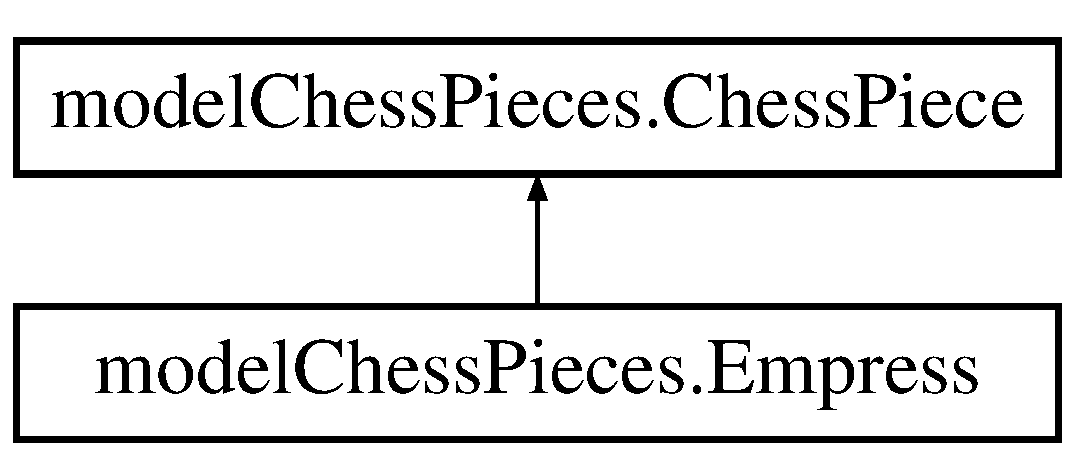
\includegraphics[height=2.000000cm]{classmodel_chess_pieces_1_1_empress}
\end{center}
\end{figure}
\subsection*{Public Member Functions}
\begin{DoxyCompactItemize}
\item 
\hyperlink{classmodel_chess_pieces_1_1_empress_a6e3bd690dae8ab6f26ece63c27f0e144}{Empress} (String \hyperlink{classmodel_chess_pieces_1_1_chess_piece_a195487ca88c197af7c1604247be31db2}{type}, int \hyperlink{classmodel_chess_pieces_1_1_chess_piece_a979e63b99128333883acedc38d25dc87}{number})
\item 
\hyperlink{classmodel_chess_pieces_1_1_empress_ac38cc0d134a721d07434d3d9b9793e30}{Empress} (String \hyperlink{classmodel_chess_pieces_1_1_chess_piece_a195487ca88c197af7c1604247be31db2}{type}, \hyperlink{classmodel_core_1_1_position}{Position} \hyperlink{classmodel_chess_pieces_1_1_chess_piece_a3d4362d5b28f6edb14161196d9c6807d}{position}, int \hyperlink{classmodel_chess_pieces_1_1_chess_piece_a979e63b99128333883acedc38d25dc87}{number})
\item 
void \hyperlink{classmodel_chess_pieces_1_1_empress_a9836219f1e3cb7ce9e809a63256192d0}{getpossible\+Next\+Positions} (\hyperlink{classmodel_core_1_1_chess_board}{Chess\+Board} chess\+Board)
\end{DoxyCompactItemize}
\subsection*{Additional Inherited Members}


\subsection{Detailed Description}
This is the class for empress \begin{DoxyAuthor}{Author}
haoranyu 
\end{DoxyAuthor}
\begin{DoxySince}{Since}
2015-\/02-\/13 01\+:19\+:26 
\end{DoxySince}
\begin{DoxyVersion}{Version}
1.\+0 
\end{DoxyVersion}


\subsection{Constructor \& Destructor Documentation}
\hypertarget{classmodel_chess_pieces_1_1_empress_a6e3bd690dae8ab6f26ece63c27f0e144}{\index{model\+Chess\+Pieces\+::\+Empress@{model\+Chess\+Pieces\+::\+Empress}!Empress@{Empress}}
\index{Empress@{Empress}!model\+Chess\+Pieces\+::\+Empress@{model\+Chess\+Pieces\+::\+Empress}}
\subsubsection[{Empress}]{\setlength{\rightskip}{0pt plus 5cm}model\+Chess\+Pieces.\+Empress.\+Empress (
\begin{DoxyParamCaption}
\item[{String}]{type, }
\item[{int}]{number}
\end{DoxyParamCaption}
)}}\label{classmodel_chess_pieces_1_1_empress_a6e3bd690dae8ab6f26ece63c27f0e144}
Constructor for default \hyperlink{classmodel_chess_pieces_1_1_empress}{Empress}


\begin{DoxyParams}{Parameters}
{\em type} & the color or null \\
\hline
{\em number} & the numbering of empress \\
\hline
\end{DoxyParams}
\hypertarget{classmodel_chess_pieces_1_1_empress_ac38cc0d134a721d07434d3d9b9793e30}{\index{model\+Chess\+Pieces\+::\+Empress@{model\+Chess\+Pieces\+::\+Empress}!Empress@{Empress}}
\index{Empress@{Empress}!model\+Chess\+Pieces\+::\+Empress@{model\+Chess\+Pieces\+::\+Empress}}
\subsubsection[{Empress}]{\setlength{\rightskip}{0pt plus 5cm}model\+Chess\+Pieces.\+Empress.\+Empress (
\begin{DoxyParamCaption}
\item[{String}]{type, }
\item[{{\bf Position}}]{position, }
\item[{int}]{number}
\end{DoxyParamCaption}
)}}\label{classmodel_chess_pieces_1_1_empress_ac38cc0d134a721d07434d3d9b9793e30}
Constructor for \hyperlink{classmodel_chess_pieces_1_1_empress}{Empress} with specified position


\begin{DoxyParams}{Parameters}
{\em type} & the color or null \\
\hline
{\em position} & the position of this knight \\
\hline
{\em number} & the numbering of knight \\
\hline
\end{DoxyParams}


\subsection{Member Function Documentation}
\hypertarget{classmodel_chess_pieces_1_1_empress_a9836219f1e3cb7ce9e809a63256192d0}{\index{model\+Chess\+Pieces\+::\+Empress@{model\+Chess\+Pieces\+::\+Empress}!getpossible\+Next\+Positions@{getpossible\+Next\+Positions}}
\index{getpossible\+Next\+Positions@{getpossible\+Next\+Positions}!model\+Chess\+Pieces\+::\+Empress@{model\+Chess\+Pieces\+::\+Empress}}
\subsubsection[{getpossible\+Next\+Positions}]{\setlength{\rightskip}{0pt plus 5cm}void model\+Chess\+Pieces.\+Empress.\+getpossible\+Next\+Positions (
\begin{DoxyParamCaption}
\item[{{\bf Chess\+Board}}]{chess\+Board}
\end{DoxyParamCaption}
)}}\label{classmodel_chess_pieces_1_1_empress_a9836219f1e3cb7ce9e809a63256192d0}
Get all possible position for the next step


\begin{DoxyParams}{Parameters}
{\em chess\+Board} & the chess board we are now on \\
\hline
\end{DoxyParams}


The documentation for this class was generated from the following file\+:\begin{DoxyCompactItemize}
\item 
src/model\+Chess\+Pieces/Empress.\+java\end{DoxyCompactItemize}

\hypertarget{classmodel_chess_pieces_1_1_empty}{\section{model\+Chess\+Pieces.\+Empty Class Reference}
\label{classmodel_chess_pieces_1_1_empty}\index{model\+Chess\+Pieces.\+Empty@{model\+Chess\+Pieces.\+Empty}}
}
Inheritance diagram for model\+Chess\+Pieces.\+Empty\+:\begin{figure}[H]
\begin{center}
\leavevmode
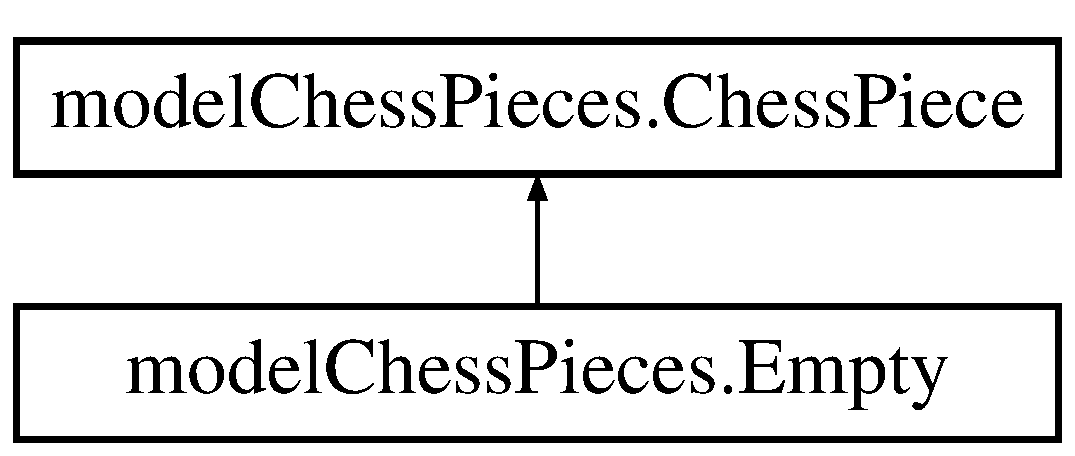
\includegraphics[height=2.000000cm]{classmodel_chess_pieces_1_1_empty}
\end{center}
\end{figure}
\subsection*{Public Member Functions}
\begin{DoxyCompactItemize}
\item 
void \hyperlink{classmodel_chess_pieces_1_1_empty_a9a52629a6d66359c933cf08e96bb6456}{get\+Possible\+Next\+Positions} (\hyperlink{classmodel_core_1_1_chess_board}{Chess\+Board} chess\+Board)
\end{DoxyCompactItemize}
\subsection*{Additional Inherited Members}


\subsection{Detailed Description}
This is the class for no chess piece (a special chess piece called \hyperlink{classmodel_chess_pieces_1_1_empty}{Empty}) Any empty cell in the chess board will be viewed as empty chess piece. \begin{DoxyAuthor}{Author}
haoranyu 
\end{DoxyAuthor}
\begin{DoxySince}{Since}
2015-\/02-\/13 01\+:19\+:17 
\end{DoxySince}
\begin{DoxyVersion}{Version}
1.\+0 
\end{DoxyVersion}


\subsection{Member Function Documentation}
\hypertarget{classmodel_chess_pieces_1_1_empty_a9a52629a6d66359c933cf08e96bb6456}{\index{model\+Chess\+Pieces\+::\+Empty@{model\+Chess\+Pieces\+::\+Empty}!get\+Possible\+Next\+Positions@{get\+Possible\+Next\+Positions}}
\index{get\+Possible\+Next\+Positions@{get\+Possible\+Next\+Positions}!model\+Chess\+Pieces\+::\+Empty@{model\+Chess\+Pieces\+::\+Empty}}
\subsubsection[{get\+Possible\+Next\+Positions}]{\setlength{\rightskip}{0pt plus 5cm}void model\+Chess\+Pieces.\+Empty.\+get\+Possible\+Next\+Positions (
\begin{DoxyParamCaption}
\item[{{\bf Chess\+Board}}]{chess\+Board}
\end{DoxyParamCaption}
)}}\label{classmodel_chess_pieces_1_1_empty_a9a52629a6d66359c933cf08e96bb6456}
Get all possible position for the next step


\begin{DoxyParams}{Parameters}
{\em chess\+Board} & the chess board we are now on \\
\hline
\end{DoxyParams}


The documentation for this class was generated from the following file\+:\begin{DoxyCompactItemize}
\item 
src/model\+Chess\+Pieces/Empty.\+java\end{DoxyCompactItemize}

\hypertarget{classmodel_chess_pieces_1_1_king}{\section{model\+Chess\+Pieces.\+King Class Reference}
\label{classmodel_chess_pieces_1_1_king}\index{model\+Chess\+Pieces.\+King@{model\+Chess\+Pieces.\+King}}
}
Inheritance diagram for model\+Chess\+Pieces.\+King\+:\begin{figure}[H]
\begin{center}
\leavevmode
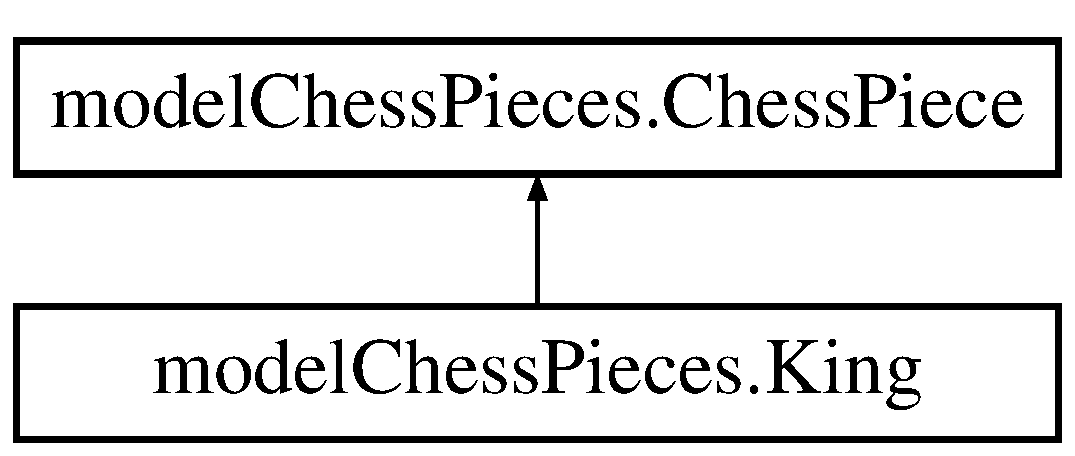
\includegraphics[height=2.000000cm]{classmodel_chess_pieces_1_1_king}
\end{center}
\end{figure}
\subsection*{Public Member Functions}
\begin{DoxyCompactItemize}
\item 
\hyperlink{classmodel_chess_pieces_1_1_king_addca0068eced10beccbb62407358e10a}{King} (String \hyperlink{classmodel_chess_pieces_1_1_chess_piece_a195487ca88c197af7c1604247be31db2}{type})
\item 
\hyperlink{classmodel_chess_pieces_1_1_king_a304e8f6364f887674d05a98e7a6f3ea1}{King} (String \hyperlink{classmodel_chess_pieces_1_1_chess_piece_a195487ca88c197af7c1604247be31db2}{type}, \hyperlink{classmodel_core_1_1_position}{Position} \hyperlink{classmodel_chess_pieces_1_1_chess_piece_a3d4362d5b28f6edb14161196d9c6807d}{position})
\item 
void \hyperlink{classmodel_chess_pieces_1_1_king_a2e7719a816495c0fae7188c3d96a2213}{getpossible\+Next\+Positions} (\hyperlink{classmodel_core_1_1_chess_board}{Chess\+Board} chess\+Board)
\end{DoxyCompactItemize}
\subsection*{Additional Inherited Members}


\subsection{Detailed Description}
This is the class for king \begin{DoxyAuthor}{Author}
haoranyu 
\end{DoxyAuthor}
\begin{DoxySince}{Since}
2015-\/02-\/13 01\+:19\+:22 
\end{DoxySince}
\begin{DoxyVersion}{Version}
1.\+0 
\end{DoxyVersion}


\subsection{Constructor \& Destructor Documentation}
\hypertarget{classmodel_chess_pieces_1_1_king_addca0068eced10beccbb62407358e10a}{\index{model\+Chess\+Pieces\+::\+King@{model\+Chess\+Pieces\+::\+King}!King@{King}}
\index{King@{King}!model\+Chess\+Pieces\+::\+King@{model\+Chess\+Pieces\+::\+King}}
\subsubsection[{King}]{\setlength{\rightskip}{0pt plus 5cm}model\+Chess\+Pieces.\+King.\+King (
\begin{DoxyParamCaption}
\item[{String}]{type}
\end{DoxyParamCaption}
)}}\label{classmodel_chess_pieces_1_1_king_addca0068eced10beccbb62407358e10a}
Constructor for default \hyperlink{classmodel_chess_pieces_1_1_king}{King}


\begin{DoxyParams}{Parameters}
{\em type} & the color or null \\
\hline
\end{DoxyParams}
\hypertarget{classmodel_chess_pieces_1_1_king_a304e8f6364f887674d05a98e7a6f3ea1}{\index{model\+Chess\+Pieces\+::\+King@{model\+Chess\+Pieces\+::\+King}!King@{King}}
\index{King@{King}!model\+Chess\+Pieces\+::\+King@{model\+Chess\+Pieces\+::\+King}}
\subsubsection[{King}]{\setlength{\rightskip}{0pt plus 5cm}model\+Chess\+Pieces.\+King.\+King (
\begin{DoxyParamCaption}
\item[{String}]{type, }
\item[{{\bf Position}}]{position}
\end{DoxyParamCaption}
)}}\label{classmodel_chess_pieces_1_1_king_a304e8f6364f887674d05a98e7a6f3ea1}
Constructor for \hyperlink{classmodel_chess_pieces_1_1_king}{King} with specified position


\begin{DoxyParams}{Parameters}
{\em type} & the color or null \\
\hline
{\em position} & the position of this king \\
\hline
\end{DoxyParams}


\subsection{Member Function Documentation}
\hypertarget{classmodel_chess_pieces_1_1_king_a2e7719a816495c0fae7188c3d96a2213}{\index{model\+Chess\+Pieces\+::\+King@{model\+Chess\+Pieces\+::\+King}!getpossible\+Next\+Positions@{getpossible\+Next\+Positions}}
\index{getpossible\+Next\+Positions@{getpossible\+Next\+Positions}!model\+Chess\+Pieces\+::\+King@{model\+Chess\+Pieces\+::\+King}}
\subsubsection[{getpossible\+Next\+Positions}]{\setlength{\rightskip}{0pt plus 5cm}void model\+Chess\+Pieces.\+King.\+getpossible\+Next\+Positions (
\begin{DoxyParamCaption}
\item[{{\bf Chess\+Board}}]{chess\+Board}
\end{DoxyParamCaption}
)}}\label{classmodel_chess_pieces_1_1_king_a2e7719a816495c0fae7188c3d96a2213}
Get all possible position for the next step


\begin{DoxyParams}{Parameters}
{\em chess\+Board} & the chess board we are now on \\
\hline
\end{DoxyParams}


The documentation for this class was generated from the following file\+:\begin{DoxyCompactItemize}
\item 
src/model\+Chess\+Pieces/King.\+java\end{DoxyCompactItemize}

\hypertarget{classmodel_chess_pieces_1_1_knight}{\section{model\+Chess\+Pieces.\+Knight Class Reference}
\label{classmodel_chess_pieces_1_1_knight}\index{model\+Chess\+Pieces.\+Knight@{model\+Chess\+Pieces.\+Knight}}
}
Inheritance diagram for model\+Chess\+Pieces.\+Knight\+:\begin{figure}[H]
\begin{center}
\leavevmode
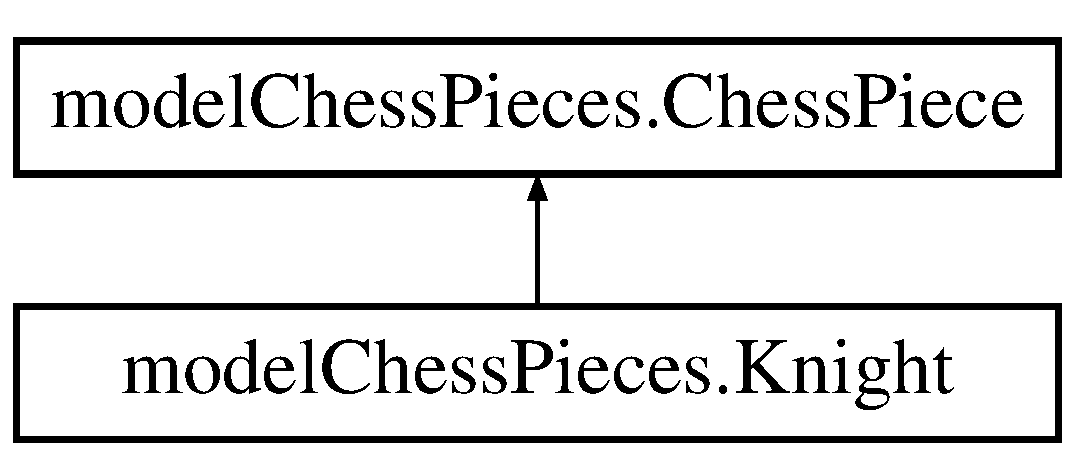
\includegraphics[height=2.000000cm]{classmodel_chess_pieces_1_1_knight}
\end{center}
\end{figure}
\subsection*{Public Member Functions}
\begin{DoxyCompactItemize}
\item 
\hyperlink{classmodel_chess_pieces_1_1_knight_a147ddcbdf9160932c8b0b386db3954eb}{Knight} (String \hyperlink{classmodel_chess_pieces_1_1_chess_piece_a195487ca88c197af7c1604247be31db2}{type}, int \hyperlink{classmodel_chess_pieces_1_1_chess_piece_a979e63b99128333883acedc38d25dc87}{number})
\item 
\hyperlink{classmodel_chess_pieces_1_1_knight_ac3d5048db997f503429d11d455db2c42}{Knight} (String \hyperlink{classmodel_chess_pieces_1_1_chess_piece_a195487ca88c197af7c1604247be31db2}{type}, \hyperlink{classmodel_core_1_1_position}{Position} \hyperlink{classmodel_chess_pieces_1_1_chess_piece_a3d4362d5b28f6edb14161196d9c6807d}{position}, int \hyperlink{classmodel_chess_pieces_1_1_chess_piece_a979e63b99128333883acedc38d25dc87}{number})
\item 
void \hyperlink{classmodel_chess_pieces_1_1_knight_aa93880a2b4001cc56b91d2afd6c17dc5}{getpossible\+Next\+Positions} (\hyperlink{classmodel_core_1_1_chess_board}{Chess\+Board} chess\+Board)
\end{DoxyCompactItemize}
\subsection*{Additional Inherited Members}


\subsection{Detailed Description}
This is the class for knight \begin{DoxyAuthor}{Author}
haoranyu 
\end{DoxyAuthor}
\begin{DoxySince}{Since}
2015-\/02-\/13 01\+:19\+:26 
\end{DoxySince}
\begin{DoxyVersion}{Version}
1.\+0 
\end{DoxyVersion}


\subsection{Constructor \& Destructor Documentation}
\hypertarget{classmodel_chess_pieces_1_1_knight_a147ddcbdf9160932c8b0b386db3954eb}{\index{model\+Chess\+Pieces\+::\+Knight@{model\+Chess\+Pieces\+::\+Knight}!Knight@{Knight}}
\index{Knight@{Knight}!model\+Chess\+Pieces\+::\+Knight@{model\+Chess\+Pieces\+::\+Knight}}
\subsubsection[{Knight}]{\setlength{\rightskip}{0pt plus 5cm}model\+Chess\+Pieces.\+Knight.\+Knight (
\begin{DoxyParamCaption}
\item[{String}]{type, }
\item[{int}]{number}
\end{DoxyParamCaption}
)}}\label{classmodel_chess_pieces_1_1_knight_a147ddcbdf9160932c8b0b386db3954eb}
Constructor for default \hyperlink{classmodel_chess_pieces_1_1_knight}{Knight}


\begin{DoxyParams}{Parameters}
{\em type} & the color or null \\
\hline
{\em number} & the numbering of knight \\
\hline
\end{DoxyParams}
\hypertarget{classmodel_chess_pieces_1_1_knight_ac3d5048db997f503429d11d455db2c42}{\index{model\+Chess\+Pieces\+::\+Knight@{model\+Chess\+Pieces\+::\+Knight}!Knight@{Knight}}
\index{Knight@{Knight}!model\+Chess\+Pieces\+::\+Knight@{model\+Chess\+Pieces\+::\+Knight}}
\subsubsection[{Knight}]{\setlength{\rightskip}{0pt plus 5cm}model\+Chess\+Pieces.\+Knight.\+Knight (
\begin{DoxyParamCaption}
\item[{String}]{type, }
\item[{{\bf Position}}]{position, }
\item[{int}]{number}
\end{DoxyParamCaption}
)}}\label{classmodel_chess_pieces_1_1_knight_ac3d5048db997f503429d11d455db2c42}
Constructor for \hyperlink{classmodel_chess_pieces_1_1_knight}{Knight} with specified position


\begin{DoxyParams}{Parameters}
{\em type} & the color or null \\
\hline
{\em position} & the position of this knight \\
\hline
{\em number} & the numbering of knight \\
\hline
\end{DoxyParams}


\subsection{Member Function Documentation}
\hypertarget{classmodel_chess_pieces_1_1_knight_aa93880a2b4001cc56b91d2afd6c17dc5}{\index{model\+Chess\+Pieces\+::\+Knight@{model\+Chess\+Pieces\+::\+Knight}!getpossible\+Next\+Positions@{getpossible\+Next\+Positions}}
\index{getpossible\+Next\+Positions@{getpossible\+Next\+Positions}!model\+Chess\+Pieces\+::\+Knight@{model\+Chess\+Pieces\+::\+Knight}}
\subsubsection[{getpossible\+Next\+Positions}]{\setlength{\rightskip}{0pt plus 5cm}void model\+Chess\+Pieces.\+Knight.\+getpossible\+Next\+Positions (
\begin{DoxyParamCaption}
\item[{{\bf Chess\+Board}}]{chess\+Board}
\end{DoxyParamCaption}
)}}\label{classmodel_chess_pieces_1_1_knight_aa93880a2b4001cc56b91d2afd6c17dc5}
Get all possible position for the next step


\begin{DoxyParams}{Parameters}
{\em chess\+Board} & the chess board we are now on \\
\hline
\end{DoxyParams}


The documentation for this class was generated from the following file\+:\begin{DoxyCompactItemize}
\item 
src/model\+Chess\+Pieces/Knight.\+java\end{DoxyCompactItemize}

\hypertarget{classmodel_chess_pieces_1_1_pawn}{\section{model\+Chess\+Pieces.\+Pawn Class Reference}
\label{classmodel_chess_pieces_1_1_pawn}\index{model\+Chess\+Pieces.\+Pawn@{model\+Chess\+Pieces.\+Pawn}}
}
Inheritance diagram for model\+Chess\+Pieces.\+Pawn\+:\begin{figure}[H]
\begin{center}
\leavevmode
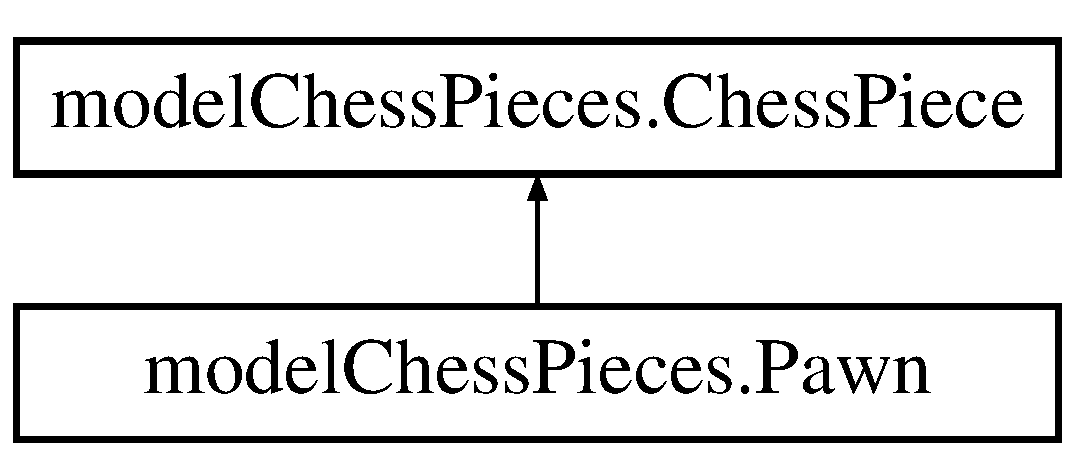
\includegraphics[height=2.000000cm]{classmodel_chess_pieces_1_1_pawn}
\end{center}
\end{figure}
\subsection*{Public Member Functions}
\begin{DoxyCompactItemize}
\item 
\hyperlink{classmodel_chess_pieces_1_1_pawn_a7621de9604258a4ec1c58480b1655564}{Pawn} (String \hyperlink{classmodel_chess_pieces_1_1_chess_piece_a195487ca88c197af7c1604247be31db2}{type}, int \hyperlink{classmodel_chess_pieces_1_1_chess_piece_a979e63b99128333883acedc38d25dc87}{number})
\item 
\hyperlink{classmodel_chess_pieces_1_1_pawn_afcf3ca5e22f454c225ca2240af0f4519}{Pawn} (String \hyperlink{classmodel_chess_pieces_1_1_chess_piece_a195487ca88c197af7c1604247be31db2}{type}, \hyperlink{classmodel_core_1_1_position}{Position} \hyperlink{classmodel_chess_pieces_1_1_chess_piece_a3d4362d5b28f6edb14161196d9c6807d}{position}, int \hyperlink{classmodel_chess_pieces_1_1_chess_piece_a979e63b99128333883acedc38d25dc87}{number})
\item 
void \hyperlink{classmodel_chess_pieces_1_1_pawn_a5d8959f38fa543fc471ca95b025cea91}{get\+Possible\+Next\+Positions} (\hyperlink{classmodel_core_1_1_chess_board}{Chess\+Board} chess\+Board)
\end{DoxyCompactItemize}
\subsection*{Protected Member Functions}
\begin{DoxyCompactItemize}
\item 
boolean \hyperlink{classmodel_chess_pieces_1_1_pawn_adf484645070f9dd3a774ea779aa84260}{add\+If\+Avaliable} (\hyperlink{classmodel_core_1_1_chess_board}{Chess\+Board} chess\+Board, \hyperlink{classmodel_core_1_1_position}{Position} \hyperlink{classmodel_chess_pieces_1_1_chess_piece_a3d4362d5b28f6edb14161196d9c6807d}{position})
\end{DoxyCompactItemize}
\subsection*{Additional Inherited Members}


\subsection{Detailed Description}
This is the class for pawn \begin{DoxyAuthor}{Author}
haoranyu 
\end{DoxyAuthor}
\begin{DoxySince}{Since}
2015-\/02-\/13 16\+:48\+:36 
\end{DoxySince}
\begin{DoxyVersion}{Version}
1.\+0 
\end{DoxyVersion}


\subsection{Constructor \& Destructor Documentation}
\hypertarget{classmodel_chess_pieces_1_1_pawn_a7621de9604258a4ec1c58480b1655564}{\index{model\+Chess\+Pieces\+::\+Pawn@{model\+Chess\+Pieces\+::\+Pawn}!Pawn@{Pawn}}
\index{Pawn@{Pawn}!model\+Chess\+Pieces\+::\+Pawn@{model\+Chess\+Pieces\+::\+Pawn}}
\subsubsection[{Pawn}]{\setlength{\rightskip}{0pt plus 5cm}model\+Chess\+Pieces.\+Pawn.\+Pawn (
\begin{DoxyParamCaption}
\item[{String}]{type, }
\item[{int}]{number}
\end{DoxyParamCaption}
)}}\label{classmodel_chess_pieces_1_1_pawn_a7621de9604258a4ec1c58480b1655564}
Constructor for default \hyperlink{classmodel_chess_pieces_1_1_pawn}{Pawn}


\begin{DoxyParams}{Parameters}
{\em type} & the color or null \\
\hline
{\em number} & the numbering of pawn \\
\hline
\end{DoxyParams}
\hypertarget{classmodel_chess_pieces_1_1_pawn_afcf3ca5e22f454c225ca2240af0f4519}{\index{model\+Chess\+Pieces\+::\+Pawn@{model\+Chess\+Pieces\+::\+Pawn}!Pawn@{Pawn}}
\index{Pawn@{Pawn}!model\+Chess\+Pieces\+::\+Pawn@{model\+Chess\+Pieces\+::\+Pawn}}
\subsubsection[{Pawn}]{\setlength{\rightskip}{0pt plus 5cm}model\+Chess\+Pieces.\+Pawn.\+Pawn (
\begin{DoxyParamCaption}
\item[{String}]{type, }
\item[{{\bf Position}}]{position, }
\item[{int}]{number}
\end{DoxyParamCaption}
)}}\label{classmodel_chess_pieces_1_1_pawn_afcf3ca5e22f454c225ca2240af0f4519}
Constructor for \hyperlink{classmodel_chess_pieces_1_1_pawn}{Pawn} with specified position


\begin{DoxyParams}{Parameters}
{\em type} & the color or null \\
\hline
{\em position} & the position of this pawn \\
\hline
{\em number} & the numbering of pawn \\
\hline
\end{DoxyParams}


\subsection{Member Function Documentation}
\hypertarget{classmodel_chess_pieces_1_1_pawn_adf484645070f9dd3a774ea779aa84260}{\index{model\+Chess\+Pieces\+::\+Pawn@{model\+Chess\+Pieces\+::\+Pawn}!add\+If\+Avaliable@{add\+If\+Avaliable}}
\index{add\+If\+Avaliable@{add\+If\+Avaliable}!model\+Chess\+Pieces\+::\+Pawn@{model\+Chess\+Pieces\+::\+Pawn}}
\subsubsection[{add\+If\+Avaliable}]{\setlength{\rightskip}{0pt plus 5cm}boolean model\+Chess\+Pieces.\+Pawn.\+add\+If\+Avaliable (
\begin{DoxyParamCaption}
\item[{{\bf Chess\+Board}}]{chess\+Board, }
\item[{{\bf Position}}]{position}
\end{DoxyParamCaption}
)\hspace{0.3cm}{\ttfamily [protected]}}}\label{classmodel_chess_pieces_1_1_pawn_adf484645070f9dd3a774ea779aa84260}
This override for \hyperlink{classmodel_chess_pieces_1_1_pawn}{Pawn} case which is special If the cell is valid A\+N\+D is not self-\/occupied A\+N\+D not duplicates, Then add to possible position


\begin{DoxyParams}{Parameters}
{\em chess\+Board} & The object of chess board \\
\hline
{\em position} & The position we see into \\
\hline
\end{DoxyParams}
\hypertarget{classmodel_chess_pieces_1_1_pawn_a5d8959f38fa543fc471ca95b025cea91}{\index{model\+Chess\+Pieces\+::\+Pawn@{model\+Chess\+Pieces\+::\+Pawn}!get\+Possible\+Next\+Positions@{get\+Possible\+Next\+Positions}}
\index{get\+Possible\+Next\+Positions@{get\+Possible\+Next\+Positions}!model\+Chess\+Pieces\+::\+Pawn@{model\+Chess\+Pieces\+::\+Pawn}}
\subsubsection[{get\+Possible\+Next\+Positions}]{\setlength{\rightskip}{0pt plus 5cm}void model\+Chess\+Pieces.\+Pawn.\+get\+Possible\+Next\+Positions (
\begin{DoxyParamCaption}
\item[{{\bf Chess\+Board}}]{chess\+Board}
\end{DoxyParamCaption}
)}}\label{classmodel_chess_pieces_1_1_pawn_a5d8959f38fa543fc471ca95b025cea91}
Get all possible position for the next step


\begin{DoxyParams}{Parameters}
{\em chess\+Board} & the chess board we are now on \\
\hline
\end{DoxyParams}


The documentation for this class was generated from the following file\+:\begin{DoxyCompactItemize}
\item 
src/model\+Chess\+Pieces/Pawn.\+java\end{DoxyCompactItemize}

\hypertarget{classmodel_core_1_1_position}{\section{model\+Core.\+Position Class Reference}
\label{classmodel_core_1_1_position}\index{model\+Core.\+Position@{model\+Core.\+Position}}
}
\subsection*{Public Member Functions}
\begin{DoxyCompactItemize}
\item 
\hyperlink{classmodel_core_1_1_position_a689df995977dd8da01d733c5b0940e8b}{Position} ()
\item 
\hyperlink{classmodel_core_1_1_position_aaf7d9f851733f7e4361eadab881b5d1e}{Position} (\hyperlink{classmodel_core_1_1_position}{Position} position)
\item 
\hyperlink{classmodel_core_1_1_position_a9a5ab27a476a183a12f14b9644a74063}{Position} (int row, int col)
\item 
\hyperlink{classmodel_core_1_1_position}{Position} \hyperlink{classmodel_core_1_1_position_a414339238322766507ee2ce61e4f18fc}{get\+Right} (int step)
\item 
\hyperlink{classmodel_core_1_1_position}{Position} \hyperlink{classmodel_core_1_1_position_a43c2653aa7b9bd2ece8a746aa488e890}{get\+Left} (int step)
\item 
\hyperlink{classmodel_core_1_1_position}{Position} \hyperlink{classmodel_core_1_1_position_a922189e8018dd157a322dd55581ccd19}{get\+Up} (int step)
\item 
\hyperlink{classmodel_core_1_1_position}{Position} \hyperlink{classmodel_core_1_1_position_ad22eb535ce11e1ca0a846a98c37e2b43}{get\+Down} (int step)
\item 
void \hyperlink{classmodel_core_1_1_position_aa88918fe5d6446eb3c9f04c0b1ba92d0}{show} ()
\item 
boolean \hyperlink{classmodel_core_1_1_position_aeb1285fd0e8aa11728692d3a40c644f5}{valid} (\hyperlink{classmodel_core_1_1_chess_board}{Chess\+Board} chess\+Board)
\item 
boolean \hyperlink{classmodel_core_1_1_position_ad6cd6dc938426f8e328374e6130e51a6}{equals} (Object object)
\item 
int \hyperlink{classmodel_core_1_1_position_a87f61d46274b310c7c4edae150f20d89}{hash\+Code} ()
\item 
int \hyperlink{classmodel_core_1_1_position_a2e369524c690d77e4fe5a2f387d6351c}{get\+Col} ()
\end{DoxyCompactItemize}


\subsection{Detailed Description}
This is the class for position on the chess board \begin{DoxyAuthor}{Author}
haoranyu 
\end{DoxyAuthor}
\begin{DoxySince}{Since}
2015-\/02-\/13 01\+:19\+:47 
\end{DoxySince}
\begin{DoxyVersion}{Version}
1.\+0 
\end{DoxyVersion}


\subsection{Constructor \& Destructor Documentation}
\hypertarget{classmodel_core_1_1_position_a689df995977dd8da01d733c5b0940e8b}{\index{model\+Core\+::\+Position@{model\+Core\+::\+Position}!Position@{Position}}
\index{Position@{Position}!model\+Core\+::\+Position@{model\+Core\+::\+Position}}
\subsubsection[{Position}]{\setlength{\rightskip}{0pt plus 5cm}model\+Core.\+Position.\+Position (
\begin{DoxyParamCaption}
{}
\end{DoxyParamCaption}
)}}\label{classmodel_core_1_1_position_a689df995977dd8da01d733c5b0940e8b}
Constructor with no parameters Get a position without meaning \hypertarget{classmodel_core_1_1_position_aaf7d9f851733f7e4361eadab881b5d1e}{\index{model\+Core\+::\+Position@{model\+Core\+::\+Position}!Position@{Position}}
\index{Position@{Position}!model\+Core\+::\+Position@{model\+Core\+::\+Position}}
\subsubsection[{Position}]{\setlength{\rightskip}{0pt plus 5cm}model\+Core.\+Position.\+Position (
\begin{DoxyParamCaption}
\item[{{\bf Position}}]{position}
\end{DoxyParamCaption}
)}}\label{classmodel_core_1_1_position_aaf7d9f851733f7e4361eadab881b5d1e}
Copy constructor


\begin{DoxyParams}{Parameters}
{\em position} & The position to copy from \\
\hline
\end{DoxyParams}
\hypertarget{classmodel_core_1_1_position_a9a5ab27a476a183a12f14b9644a74063}{\index{model\+Core\+::\+Position@{model\+Core\+::\+Position}!Position@{Position}}
\index{Position@{Position}!model\+Core\+::\+Position@{model\+Core\+::\+Position}}
\subsubsection[{Position}]{\setlength{\rightskip}{0pt plus 5cm}model\+Core.\+Position.\+Position (
\begin{DoxyParamCaption}
\item[{int}]{row, }
\item[{int}]{col}
\end{DoxyParamCaption}
)}}\label{classmodel_core_1_1_position_a9a5ab27a476a183a12f14b9644a74063}
Constructor of \hyperlink{classmodel_core_1_1_position}{Position} with initial row and column


\begin{DoxyParams}{Parameters}
{\em row} & The row of position to initialize from \\
\hline
{\em col} & The column of position to initialize from \\
\hline
\end{DoxyParams}


\subsection{Member Function Documentation}
\hypertarget{classmodel_core_1_1_position_ad6cd6dc938426f8e328374e6130e51a6}{\index{model\+Core\+::\+Position@{model\+Core\+::\+Position}!equals@{equals}}
\index{equals@{equals}!model\+Core\+::\+Position@{model\+Core\+::\+Position}}
\subsubsection[{equals}]{\setlength{\rightskip}{0pt plus 5cm}boolean model\+Core.\+Position.\+equals (
\begin{DoxyParamCaption}
\item[{Object}]{object}
\end{DoxyParamCaption}
)}}\label{classmodel_core_1_1_position_ad6cd6dc938426f8e328374e6130e51a6}
Override original equals function

\begin{DoxySeeAlso}{See also}
java.\+lang.\+Object\+::equals(java.\+lang.\+Object) 
\end{DoxySeeAlso}
\hypertarget{classmodel_core_1_1_position_a2e369524c690d77e4fe5a2f387d6351c}{\index{model\+Core\+::\+Position@{model\+Core\+::\+Position}!get\+Col@{get\+Col}}
\index{get\+Col@{get\+Col}!model\+Core\+::\+Position@{model\+Core\+::\+Position}}
\subsubsection[{get\+Col}]{\setlength{\rightskip}{0pt plus 5cm}int model\+Core.\+Position.\+get\+Col (
\begin{DoxyParamCaption}
{}
\end{DoxyParamCaption}
)}}\label{classmodel_core_1_1_position_a2e369524c690d77e4fe5a2f387d6351c}
\begin{DoxyReturn}{Returns}
the col 
\end{DoxyReturn}
\hypertarget{classmodel_core_1_1_position_ad22eb535ce11e1ca0a846a98c37e2b43}{\index{model\+Core\+::\+Position@{model\+Core\+::\+Position}!get\+Down@{get\+Down}}
\index{get\+Down@{get\+Down}!model\+Core\+::\+Position@{model\+Core\+::\+Position}}
\subsubsection[{get\+Down}]{\setlength{\rightskip}{0pt plus 5cm}{\bf Position} model\+Core.\+Position.\+get\+Down (
\begin{DoxyParamCaption}
\item[{int}]{step}
\end{DoxyParamCaption}
)}}\label{classmodel_core_1_1_position_ad22eb535ce11e1ca0a846a98c37e2b43}
Get the position to number of step away to the bottom


\begin{DoxyParams}{Parameters}
{\em step} & The number of steps \\
\hline
\end{DoxyParams}
\begin{DoxyReturn}{Returns}
The new position after calucation 
\end{DoxyReturn}
\hypertarget{classmodel_core_1_1_position_a43c2653aa7b9bd2ece8a746aa488e890}{\index{model\+Core\+::\+Position@{model\+Core\+::\+Position}!get\+Left@{get\+Left}}
\index{get\+Left@{get\+Left}!model\+Core\+::\+Position@{model\+Core\+::\+Position}}
\subsubsection[{get\+Left}]{\setlength{\rightskip}{0pt plus 5cm}{\bf Position} model\+Core.\+Position.\+get\+Left (
\begin{DoxyParamCaption}
\item[{int}]{step}
\end{DoxyParamCaption}
)}}\label{classmodel_core_1_1_position_a43c2653aa7b9bd2ece8a746aa488e890}
Get the position to number of step away to the left


\begin{DoxyParams}{Parameters}
{\em step} & The number of steps \\
\hline
\end{DoxyParams}
\begin{DoxyReturn}{Returns}
The new position after calucation 
\end{DoxyReturn}
\hypertarget{classmodel_core_1_1_position_a414339238322766507ee2ce61e4f18fc}{\index{model\+Core\+::\+Position@{model\+Core\+::\+Position}!get\+Right@{get\+Right}}
\index{get\+Right@{get\+Right}!model\+Core\+::\+Position@{model\+Core\+::\+Position}}
\subsubsection[{get\+Right}]{\setlength{\rightskip}{0pt plus 5cm}{\bf Position} model\+Core.\+Position.\+get\+Right (
\begin{DoxyParamCaption}
\item[{int}]{step}
\end{DoxyParamCaption}
)}}\label{classmodel_core_1_1_position_a414339238322766507ee2ce61e4f18fc}
Get the position to number of step away to the right


\begin{DoxyParams}{Parameters}
{\em step} & The number of steps \\
\hline
\end{DoxyParams}
\begin{DoxyReturn}{Returns}
The new position after calucation 
\end{DoxyReturn}
\hypertarget{classmodel_core_1_1_position_a922189e8018dd157a322dd55581ccd19}{\index{model\+Core\+::\+Position@{model\+Core\+::\+Position}!get\+Up@{get\+Up}}
\index{get\+Up@{get\+Up}!model\+Core\+::\+Position@{model\+Core\+::\+Position}}
\subsubsection[{get\+Up}]{\setlength{\rightskip}{0pt plus 5cm}{\bf Position} model\+Core.\+Position.\+get\+Up (
\begin{DoxyParamCaption}
\item[{int}]{step}
\end{DoxyParamCaption}
)}}\label{classmodel_core_1_1_position_a922189e8018dd157a322dd55581ccd19}
Get the position to number of step away to the top


\begin{DoxyParams}{Parameters}
{\em step} & The number of steps \\
\hline
\end{DoxyParams}
\begin{DoxyReturn}{Returns}
The new position after calucation 
\end{DoxyReturn}
\hypertarget{classmodel_core_1_1_position_a87f61d46274b310c7c4edae150f20d89}{\index{model\+Core\+::\+Position@{model\+Core\+::\+Position}!hash\+Code@{hash\+Code}}
\index{hash\+Code@{hash\+Code}!model\+Core\+::\+Position@{model\+Core\+::\+Position}}
\subsubsection[{hash\+Code}]{\setlength{\rightskip}{0pt plus 5cm}int model\+Core.\+Position.\+hash\+Code (
\begin{DoxyParamCaption}
{}
\end{DoxyParamCaption}
)}}\label{classmodel_core_1_1_position_a87f61d46274b310c7c4edae150f20d89}
Override original hash\+Code function

\begin{DoxySeeAlso}{See also}
java.\+lang.\+Object\+::hash\+Code() 
\end{DoxySeeAlso}
\hypertarget{classmodel_core_1_1_position_aa88918fe5d6446eb3c9f04c0b1ba92d0}{\index{model\+Core\+::\+Position@{model\+Core\+::\+Position}!show@{show}}
\index{show@{show}!model\+Core\+::\+Position@{model\+Core\+::\+Position}}
\subsubsection[{show}]{\setlength{\rightskip}{0pt plus 5cm}void model\+Core.\+Position.\+show (
\begin{DoxyParamCaption}
{}
\end{DoxyParamCaption}
)}}\label{classmodel_core_1_1_position_aa88918fe5d6446eb3c9f04c0b1ba92d0}
A print out help function that print the pair of position W\+I\+L\+L B\+E R\+E\+M\+O\+V\+E\+D L\+A\+T\+E\+R \hypertarget{classmodel_core_1_1_position_aeb1285fd0e8aa11728692d3a40c644f5}{\index{model\+Core\+::\+Position@{model\+Core\+::\+Position}!valid@{valid}}
\index{valid@{valid}!model\+Core\+::\+Position@{model\+Core\+::\+Position}}
\subsubsection[{valid}]{\setlength{\rightskip}{0pt plus 5cm}boolean model\+Core.\+Position.\+valid (
\begin{DoxyParamCaption}
\item[{{\bf Chess\+Board}}]{chess\+Board}
\end{DoxyParamCaption}
)}}\label{classmodel_core_1_1_position_aeb1285fd0e8aa11728692d3a40c644f5}
Test whether the position is in the chess board


\begin{DoxyParams}{Parameters}
{\em chess\+Board} & The chess board we see into \\
\hline
\end{DoxyParams}
\begin{DoxyReturn}{Returns}
True if the row and column specified exist in the chess board 
\end{DoxyReturn}


The documentation for this class was generated from the following file\+:\begin{DoxyCompactItemize}
\item 
src/model\+Core/Position.\+java\end{DoxyCompactItemize}

\hypertarget{classmodel_chess_pieces_1_1_princess}{\section{model\+Chess\+Pieces.\+Princess Class Reference}
\label{classmodel_chess_pieces_1_1_princess}\index{model\+Chess\+Pieces.\+Princess@{model\+Chess\+Pieces.\+Princess}}
}
Inheritance diagram for model\+Chess\+Pieces.\+Princess\+:\begin{figure}[H]
\begin{center}
\leavevmode
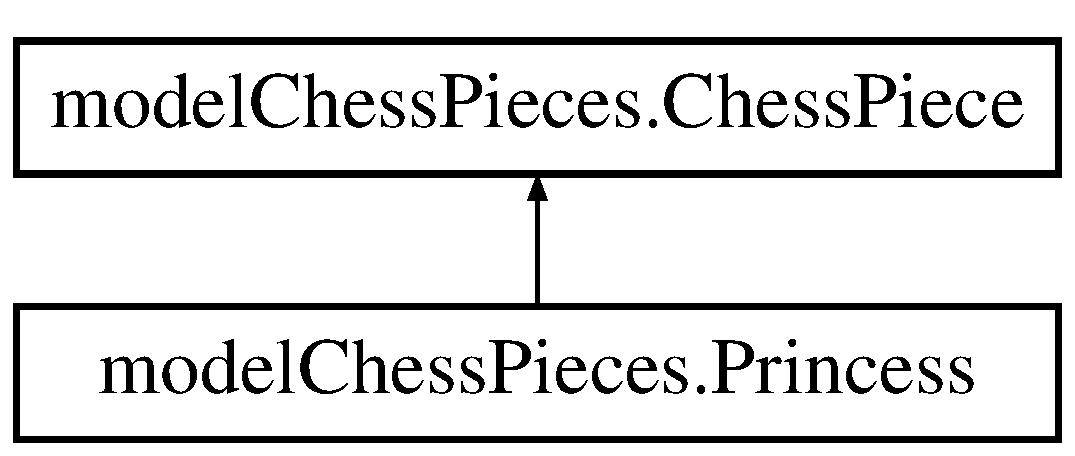
\includegraphics[height=2.000000cm]{classmodel_chess_pieces_1_1_princess}
\end{center}
\end{figure}
\subsection*{Public Member Functions}
\begin{DoxyCompactItemize}
\item 
\hyperlink{classmodel_chess_pieces_1_1_princess_a33cb1197bcb1f8808ea931626f2cf90b}{Princess} (String \hyperlink{classmodel_chess_pieces_1_1_chess_piece_a195487ca88c197af7c1604247be31db2}{type}, int \hyperlink{classmodel_chess_pieces_1_1_chess_piece_a979e63b99128333883acedc38d25dc87}{number})
\item 
\hyperlink{classmodel_chess_pieces_1_1_princess_a4c6de589407a7e236d78a89cffd41b97}{Princess} (String \hyperlink{classmodel_chess_pieces_1_1_chess_piece_a195487ca88c197af7c1604247be31db2}{type}, \hyperlink{classmodel_core_1_1_position}{Position} \hyperlink{classmodel_chess_pieces_1_1_chess_piece_a3d4362d5b28f6edb14161196d9c6807d}{position}, int \hyperlink{classmodel_chess_pieces_1_1_chess_piece_a979e63b99128333883acedc38d25dc87}{number})
\item 
void \hyperlink{classmodel_chess_pieces_1_1_princess_aa7c8b759767abcfc81e9e5ba74ac0bc0}{get\+Possible\+Next\+Position} (\hyperlink{classmodel_core_1_1_chess_board}{Chess\+Board} chess\+Board)
\end{DoxyCompactItemize}
\subsection*{Additional Inherited Members}


\subsection{Detailed Description}
This is the class for princess \begin{DoxyAuthor}{Author}
haoranyu 
\end{DoxyAuthor}
\begin{DoxySince}{Since}
2015-\/02-\/13 01\+:19\+:26 
\end{DoxySince}
\begin{DoxyVersion}{Version}
1.\+0 
\end{DoxyVersion}


\subsection{Constructor \& Destructor Documentation}
\hypertarget{classmodel_chess_pieces_1_1_princess_a33cb1197bcb1f8808ea931626f2cf90b}{\index{model\+Chess\+Pieces\+::\+Princess@{model\+Chess\+Pieces\+::\+Princess}!Princess@{Princess}}
\index{Princess@{Princess}!model\+Chess\+Pieces\+::\+Princess@{model\+Chess\+Pieces\+::\+Princess}}
\subsubsection[{Princess}]{\setlength{\rightskip}{0pt plus 5cm}model\+Chess\+Pieces.\+Princess.\+Princess (
\begin{DoxyParamCaption}
\item[{String}]{type, }
\item[{int}]{number}
\end{DoxyParamCaption}
)}}\label{classmodel_chess_pieces_1_1_princess_a33cb1197bcb1f8808ea931626f2cf90b}
Constructor for default \hyperlink{classmodel_chess_pieces_1_1_princess}{Princess}


\begin{DoxyParams}{Parameters}
{\em type} & the color or null \\
\hline
{\em number} & the numbering of princess \\
\hline
\end{DoxyParams}
\hypertarget{classmodel_chess_pieces_1_1_princess_a4c6de589407a7e236d78a89cffd41b97}{\index{model\+Chess\+Pieces\+::\+Princess@{model\+Chess\+Pieces\+::\+Princess}!Princess@{Princess}}
\index{Princess@{Princess}!model\+Chess\+Pieces\+::\+Princess@{model\+Chess\+Pieces\+::\+Princess}}
\subsubsection[{Princess}]{\setlength{\rightskip}{0pt plus 5cm}model\+Chess\+Pieces.\+Princess.\+Princess (
\begin{DoxyParamCaption}
\item[{String}]{type, }
\item[{{\bf Position}}]{position, }
\item[{int}]{number}
\end{DoxyParamCaption}
)}}\label{classmodel_chess_pieces_1_1_princess_a4c6de589407a7e236d78a89cffd41b97}
Constructor for \hyperlink{classmodel_chess_pieces_1_1_princess}{Princess} with specified position


\begin{DoxyParams}{Parameters}
{\em type} & the color or null \\
\hline
{\em position} & the position of this princess \\
\hline
{\em number} & the numbering of princess \\
\hline
\end{DoxyParams}


\subsection{Member Function Documentation}
\hypertarget{classmodel_chess_pieces_1_1_princess_aa7c8b759767abcfc81e9e5ba74ac0bc0}{\index{model\+Chess\+Pieces\+::\+Princess@{model\+Chess\+Pieces\+::\+Princess}!get\+Possible\+Next\+Position@{get\+Possible\+Next\+Position}}
\index{get\+Possible\+Next\+Position@{get\+Possible\+Next\+Position}!model\+Chess\+Pieces\+::\+Princess@{model\+Chess\+Pieces\+::\+Princess}}
\subsubsection[{get\+Possible\+Next\+Position}]{\setlength{\rightskip}{0pt plus 5cm}void model\+Chess\+Pieces.\+Princess.\+get\+Possible\+Next\+Position (
\begin{DoxyParamCaption}
\item[{{\bf Chess\+Board}}]{chess\+Board}
\end{DoxyParamCaption}
)}}\label{classmodel_chess_pieces_1_1_princess_aa7c8b759767abcfc81e9e5ba74ac0bc0}
Get all possible position for the next step


\begin{DoxyParams}{Parameters}
{\em chess\+Board} & the chess board we are now on \\
\hline
\end{DoxyParams}


The documentation for this class was generated from the following file\+:\begin{DoxyCompactItemize}
\item 
src/model\+Chess\+Pieces/Princess.\+java\end{DoxyCompactItemize}

\hypertarget{classmodel_chess_pieces_1_1_queen}{\section{model\+Chess\+Pieces.\+Queen Class Reference}
\label{classmodel_chess_pieces_1_1_queen}\index{model\+Chess\+Pieces.\+Queen@{model\+Chess\+Pieces.\+Queen}}
}
Inheritance diagram for model\+Chess\+Pieces.\+Queen\+:\begin{figure}[H]
\begin{center}
\leavevmode
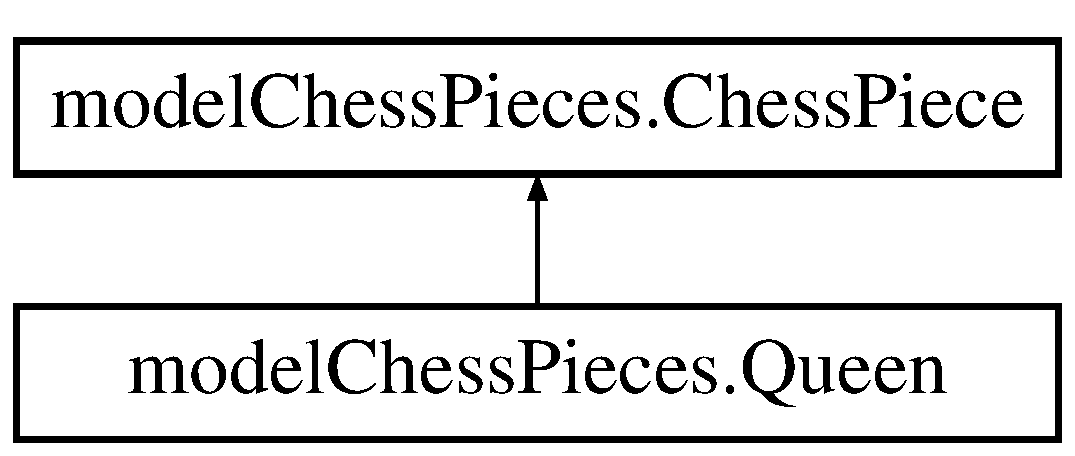
\includegraphics[height=2.000000cm]{classmodel_chess_pieces_1_1_queen}
\end{center}
\end{figure}
\subsection*{Public Member Functions}
\begin{DoxyCompactItemize}
\item 
\hyperlink{classmodel_chess_pieces_1_1_queen_a7b704ff103b506b01303c9acfc777240}{Queen} (String \hyperlink{classmodel_chess_pieces_1_1_chess_piece_a195487ca88c197af7c1604247be31db2}{type})
\item 
\hyperlink{classmodel_chess_pieces_1_1_queen_a020aae1c181f51bf9a587c35ff7388c4}{Queen} (String \hyperlink{classmodel_chess_pieces_1_1_chess_piece_a195487ca88c197af7c1604247be31db2}{type}, \hyperlink{classmodel_core_1_1_position}{Position} \hyperlink{classmodel_chess_pieces_1_1_chess_piece_a3d4362d5b28f6edb14161196d9c6807d}{position})
\item 
void \hyperlink{classmodel_chess_pieces_1_1_queen_ab5c509d5eecc67d16fcde996a90f7099}{get\+Possible\+Next\+Positions} (\hyperlink{classmodel_core_1_1_chess_board}{Chess\+Board} chess\+Board)
\end{DoxyCompactItemize}
\subsection*{Additional Inherited Members}


\subsection{Detailed Description}
This is the class for queen \begin{DoxyAuthor}{Author}
haoranyu 
\end{DoxyAuthor}
\begin{DoxySince}{Since}
2015-\/02-\/13 01\+:19\+:38 
\end{DoxySince}
\begin{DoxyVersion}{Version}
1.\+0 
\end{DoxyVersion}


\subsection{Constructor \& Destructor Documentation}
\hypertarget{classmodel_chess_pieces_1_1_queen_a7b704ff103b506b01303c9acfc777240}{\index{model\+Chess\+Pieces\+::\+Queen@{model\+Chess\+Pieces\+::\+Queen}!Queen@{Queen}}
\index{Queen@{Queen}!model\+Chess\+Pieces\+::\+Queen@{model\+Chess\+Pieces\+::\+Queen}}
\subsubsection[{Queen}]{\setlength{\rightskip}{0pt plus 5cm}model\+Chess\+Pieces.\+Queen.\+Queen (
\begin{DoxyParamCaption}
\item[{String}]{type}
\end{DoxyParamCaption}
)}}\label{classmodel_chess_pieces_1_1_queen_a7b704ff103b506b01303c9acfc777240}
Constructor for default \hyperlink{classmodel_chess_pieces_1_1_queen}{Queen}


\begin{DoxyParams}{Parameters}
{\em type} & the color or null \\
\hline
\end{DoxyParams}
\hypertarget{classmodel_chess_pieces_1_1_queen_a020aae1c181f51bf9a587c35ff7388c4}{\index{model\+Chess\+Pieces\+::\+Queen@{model\+Chess\+Pieces\+::\+Queen}!Queen@{Queen}}
\index{Queen@{Queen}!model\+Chess\+Pieces\+::\+Queen@{model\+Chess\+Pieces\+::\+Queen}}
\subsubsection[{Queen}]{\setlength{\rightskip}{0pt plus 5cm}model\+Chess\+Pieces.\+Queen.\+Queen (
\begin{DoxyParamCaption}
\item[{String}]{type, }
\item[{{\bf Position}}]{position}
\end{DoxyParamCaption}
)}}\label{classmodel_chess_pieces_1_1_queen_a020aae1c181f51bf9a587c35ff7388c4}
Constructor for \hyperlink{classmodel_chess_pieces_1_1_queen}{Queen} with specified position


\begin{DoxyParams}{Parameters}
{\em type} & the color or null \\
\hline
{\em position} & the position of this queen \\
\hline
\end{DoxyParams}


\subsection{Member Function Documentation}
\hypertarget{classmodel_chess_pieces_1_1_queen_ab5c509d5eecc67d16fcde996a90f7099}{\index{model\+Chess\+Pieces\+::\+Queen@{model\+Chess\+Pieces\+::\+Queen}!get\+Possible\+Next\+Positions@{get\+Possible\+Next\+Positions}}
\index{get\+Possible\+Next\+Positions@{get\+Possible\+Next\+Positions}!model\+Chess\+Pieces\+::\+Queen@{model\+Chess\+Pieces\+::\+Queen}}
\subsubsection[{get\+Possible\+Next\+Positions}]{\setlength{\rightskip}{0pt plus 5cm}void model\+Chess\+Pieces.\+Queen.\+get\+Possible\+Next\+Positions (
\begin{DoxyParamCaption}
\item[{{\bf Chess\+Board}}]{chess\+Board}
\end{DoxyParamCaption}
)}}\label{classmodel_chess_pieces_1_1_queen_ab5c509d5eecc67d16fcde996a90f7099}
Get all possible position for the next step


\begin{DoxyParams}{Parameters}
{\em chess\+Board} & the chess board we are now on \\
\hline
\end{DoxyParams}


The documentation for this class was generated from the following file\+:\begin{DoxyCompactItemize}
\item 
src/model\+Chess\+Pieces/Queen.\+java\end{DoxyCompactItemize}

\hypertarget{classmodel_core_1_1_record}{\section{model\+Core.\+Record Class Reference}
\label{classmodel_core_1_1_record}\index{model\+Core.\+Record@{model\+Core.\+Record}}
}
\subsection*{Public Member Functions}
\begin{DoxyCompactItemize}
\item 
\hyperlink{classmodel_core_1_1_record_a8ea296d191e5510b45eece7db72478fd}{Record} (\hyperlink{classmodel_core_1_1_position}{Position} \hyperlink{classmodel_core_1_1_record_ae7cca522f71f0fb7b5e25b9c3fe00e46}{from\+Position}, \hyperlink{classmodel_chess_pieces_1_1_chess_piece}{Chess\+Piece} \hyperlink{classmodel_core_1_1_record_a38bcd5a97552a51ac6c3e657a2d59c77}{from\+Chess\+Piece}, \hyperlink{classmodel_core_1_1_position}{Position} \hyperlink{classmodel_core_1_1_record_a9beacb5341758e83ebe459f71b6e2511}{to\+Position}, \hyperlink{classmodel_chess_pieces_1_1_chess_piece}{Chess\+Piece} \hyperlink{classmodel_core_1_1_record_abdc3856c453073728a148a4aec3a91e9}{to\+Chess\+Piece})
\end{DoxyCompactItemize}
\subsection*{Public Attributes}
\begin{DoxyCompactItemize}
\item 
\hyperlink{classmodel_core_1_1_position}{Position} \hyperlink{classmodel_core_1_1_record_ae7cca522f71f0fb7b5e25b9c3fe00e46}{from\+Position}
\item 
\hyperlink{classmodel_core_1_1_position}{Position} \hyperlink{classmodel_core_1_1_record_a9beacb5341758e83ebe459f71b6e2511}{to\+Position}
\item 
\hyperlink{classmodel_chess_pieces_1_1_chess_piece}{Chess\+Piece} \hyperlink{classmodel_core_1_1_record_a38bcd5a97552a51ac6c3e657a2d59c77}{from\+Chess\+Piece}
\item 
\hyperlink{classmodel_chess_pieces_1_1_chess_piece}{Chess\+Piece} \hyperlink{classmodel_core_1_1_record_abdc3856c453073728a148a4aec3a91e9}{to\+Chess\+Piece}
\end{DoxyCompactItemize}


\subsection{Detailed Description}
This is the class for record

\begin{DoxyAuthor}{Author}
haoranyu 
\end{DoxyAuthor}
\begin{DoxySince}{Since}
2015-\/02-\/13 01\+:19\+:51 
\end{DoxySince}
\begin{DoxyVersion}{Version}
1.\+0 
\end{DoxyVersion}


\subsection{Constructor \& Destructor Documentation}
\hypertarget{classmodel_core_1_1_record_a8ea296d191e5510b45eece7db72478fd}{\index{model\+Core\+::\+Record@{model\+Core\+::\+Record}!Record@{Record}}
\index{Record@{Record}!model\+Core\+::\+Record@{model\+Core\+::\+Record}}
\subsubsection[{Record}]{\setlength{\rightskip}{0pt plus 5cm}model\+Core.\+Record.\+Record (
\begin{DoxyParamCaption}
\item[{{\bf Position}}]{from\+Position, }
\item[{{\bf Chess\+Piece}}]{from\+Chess\+Piece, }
\item[{{\bf Position}}]{to\+Position, }
\item[{{\bf Chess\+Piece}}]{to\+Chess\+Piece}
\end{DoxyParamCaption}
)}}\label{classmodel_core_1_1_record_a8ea296d191e5510b45eece7db72478fd}
Constructor for \hyperlink{classmodel_core_1_1_record}{Record}


\begin{DoxyParams}{Parameters}
{\em from\+Position} & the starting position of movement \\
\hline
{\em from\+Chess\+Piece} & the ending position of movement \\
\hline
{\em to\+Position} & the chess piece on starting position \\
\hline
{\em to\+Chess\+Piece} & the chess piece on ending position \\
\hline
\end{DoxyParams}


\subsection{Member Data Documentation}
\hypertarget{classmodel_core_1_1_record_a38bcd5a97552a51ac6c3e657a2d59c77}{\index{model\+Core\+::\+Record@{model\+Core\+::\+Record}!from\+Chess\+Piece@{from\+Chess\+Piece}}
\index{from\+Chess\+Piece@{from\+Chess\+Piece}!model\+Core\+::\+Record@{model\+Core\+::\+Record}}
\subsubsection[{from\+Chess\+Piece}]{\setlength{\rightskip}{0pt plus 5cm}{\bf Chess\+Piece} model\+Core.\+Record.\+from\+Chess\+Piece}}\label{classmodel_core_1_1_record_a38bcd5a97552a51ac6c3e657a2d59c77}
the chess piece on starting position \hypertarget{classmodel_core_1_1_record_ae7cca522f71f0fb7b5e25b9c3fe00e46}{\index{model\+Core\+::\+Record@{model\+Core\+::\+Record}!from\+Position@{from\+Position}}
\index{from\+Position@{from\+Position}!model\+Core\+::\+Record@{model\+Core\+::\+Record}}
\subsubsection[{from\+Position}]{\setlength{\rightskip}{0pt plus 5cm}{\bf Position} model\+Core.\+Record.\+from\+Position}}\label{classmodel_core_1_1_record_ae7cca522f71f0fb7b5e25b9c3fe00e46}
the starting position of movement \hypertarget{classmodel_core_1_1_record_abdc3856c453073728a148a4aec3a91e9}{\index{model\+Core\+::\+Record@{model\+Core\+::\+Record}!to\+Chess\+Piece@{to\+Chess\+Piece}}
\index{to\+Chess\+Piece@{to\+Chess\+Piece}!model\+Core\+::\+Record@{model\+Core\+::\+Record}}
\subsubsection[{to\+Chess\+Piece}]{\setlength{\rightskip}{0pt plus 5cm}{\bf Chess\+Piece} model\+Core.\+Record.\+to\+Chess\+Piece}}\label{classmodel_core_1_1_record_abdc3856c453073728a148a4aec3a91e9}
the chess piece on ending position \hypertarget{classmodel_core_1_1_record_a9beacb5341758e83ebe459f71b6e2511}{\index{model\+Core\+::\+Record@{model\+Core\+::\+Record}!to\+Position@{to\+Position}}
\index{to\+Position@{to\+Position}!model\+Core\+::\+Record@{model\+Core\+::\+Record}}
\subsubsection[{to\+Position}]{\setlength{\rightskip}{0pt plus 5cm}{\bf Position} model\+Core.\+Record.\+to\+Position}}\label{classmodel_core_1_1_record_a9beacb5341758e83ebe459f71b6e2511}
the ending position of movement 

The documentation for this class was generated from the following file\+:\begin{DoxyCompactItemize}
\item 
src/model\+Core/Record.\+java\end{DoxyCompactItemize}

\hypertarget{classmodel_chess_pieces_1_1_rook}{\section{model\+Chess\+Pieces.\+Rook Class Reference}
\label{classmodel_chess_pieces_1_1_rook}\index{model\+Chess\+Pieces.\+Rook@{model\+Chess\+Pieces.\+Rook}}
}
Inheritance diagram for model\+Chess\+Pieces.\+Rook\+:\begin{figure}[H]
\begin{center}
\leavevmode
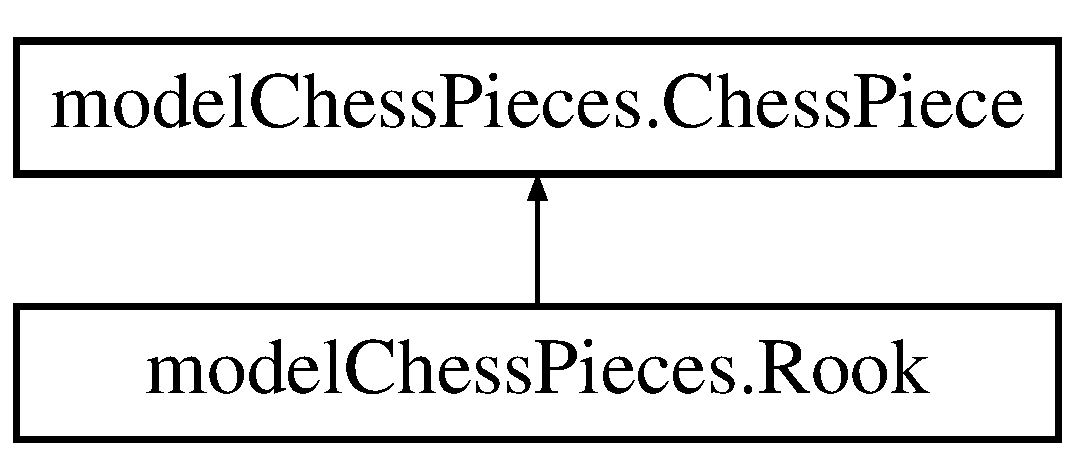
\includegraphics[height=2.000000cm]{classmodel_chess_pieces_1_1_rook}
\end{center}
\end{figure}
\subsection*{Public Member Functions}
\begin{DoxyCompactItemize}
\item 
\hyperlink{classmodel_chess_pieces_1_1_rook_a7cef743a515cb9ea132e09c99060cc96}{Rook} (String \hyperlink{classmodel_chess_pieces_1_1_chess_piece_a195487ca88c197af7c1604247be31db2}{type}, int \hyperlink{classmodel_chess_pieces_1_1_chess_piece_a979e63b99128333883acedc38d25dc87}{number})
\item 
\hyperlink{classmodel_chess_pieces_1_1_rook_af2c466d81052c7adcbb443d235aecdb6}{Rook} (String \hyperlink{classmodel_chess_pieces_1_1_chess_piece_a195487ca88c197af7c1604247be31db2}{type}, \hyperlink{classmodel_core_1_1_position}{Position} \hyperlink{classmodel_chess_pieces_1_1_chess_piece_a3d4362d5b28f6edb14161196d9c6807d}{position}, int \hyperlink{classmodel_chess_pieces_1_1_chess_piece_a979e63b99128333883acedc38d25dc87}{number})
\item 
void \hyperlink{classmodel_chess_pieces_1_1_rook_aa1dff23baf32a526be1e23cdcbe01123}{getpossible\+Next\+Positions} (\hyperlink{classmodel_core_1_1_chess_board}{Chess\+Board} chess\+Board)
\end{DoxyCompactItemize}
\subsection*{Additional Inherited Members}


\subsection{Detailed Description}
This is the class for rook \begin{DoxyAuthor}{Author}
haoranyu 
\end{DoxyAuthor}
\begin{DoxySince}{Since}
2015-\/02-\/13 01\+:19\+:42 
\end{DoxySince}
\begin{DoxyVersion}{Version}
1.\+0 
\end{DoxyVersion}


\subsection{Constructor \& Destructor Documentation}
\hypertarget{classmodel_chess_pieces_1_1_rook_a7cef743a515cb9ea132e09c99060cc96}{\index{model\+Chess\+Pieces\+::\+Rook@{model\+Chess\+Pieces\+::\+Rook}!Rook@{Rook}}
\index{Rook@{Rook}!model\+Chess\+Pieces\+::\+Rook@{model\+Chess\+Pieces\+::\+Rook}}
\subsubsection[{Rook}]{\setlength{\rightskip}{0pt plus 5cm}model\+Chess\+Pieces.\+Rook.\+Rook (
\begin{DoxyParamCaption}
\item[{String}]{type, }
\item[{int}]{number}
\end{DoxyParamCaption}
)}}\label{classmodel_chess_pieces_1_1_rook_a7cef743a515cb9ea132e09c99060cc96}
Constructor for default \hyperlink{classmodel_chess_pieces_1_1_rook}{Rook}


\begin{DoxyParams}{Parameters}
{\em type} & the color or null \\
\hline
{\em number} & the numbering of rook \\
\hline
\end{DoxyParams}
\hypertarget{classmodel_chess_pieces_1_1_rook_af2c466d81052c7adcbb443d235aecdb6}{\index{model\+Chess\+Pieces\+::\+Rook@{model\+Chess\+Pieces\+::\+Rook}!Rook@{Rook}}
\index{Rook@{Rook}!model\+Chess\+Pieces\+::\+Rook@{model\+Chess\+Pieces\+::\+Rook}}
\subsubsection[{Rook}]{\setlength{\rightskip}{0pt plus 5cm}model\+Chess\+Pieces.\+Rook.\+Rook (
\begin{DoxyParamCaption}
\item[{String}]{type, }
\item[{{\bf Position}}]{position, }
\item[{int}]{number}
\end{DoxyParamCaption}
)}}\label{classmodel_chess_pieces_1_1_rook_af2c466d81052c7adcbb443d235aecdb6}
Constructor for \hyperlink{classmodel_chess_pieces_1_1_rook}{Rook} with specified position


\begin{DoxyParams}{Parameters}
{\em type} & the color or null \\
\hline
{\em position} & the position of this rook \\
\hline
{\em number} & the numbering of rook \\
\hline
\end{DoxyParams}


\subsection{Member Function Documentation}
\hypertarget{classmodel_chess_pieces_1_1_rook_aa1dff23baf32a526be1e23cdcbe01123}{\index{model\+Chess\+Pieces\+::\+Rook@{model\+Chess\+Pieces\+::\+Rook}!getpossible\+Next\+Positions@{getpossible\+Next\+Positions}}
\index{getpossible\+Next\+Positions@{getpossible\+Next\+Positions}!model\+Chess\+Pieces\+::\+Rook@{model\+Chess\+Pieces\+::\+Rook}}
\subsubsection[{getpossible\+Next\+Positions}]{\setlength{\rightskip}{0pt plus 5cm}void model\+Chess\+Pieces.\+Rook.\+getpossible\+Next\+Positions (
\begin{DoxyParamCaption}
\item[{{\bf Chess\+Board}}]{chess\+Board}
\end{DoxyParamCaption}
)}}\label{classmodel_chess_pieces_1_1_rook_aa1dff23baf32a526be1e23cdcbe01123}
Get all possible position for the next step


\begin{DoxyParams}{Parameters}
{\em chess\+Board} & the chess board we are now on \\
\hline
\end{DoxyParams}


The documentation for this class was generated from the following file\+:\begin{DoxyCompactItemize}
\item 
src/model\+Chess\+Pieces/Rook.\+java\end{DoxyCompactItemize}

%--- End generated contents ---

% Index
\newpage
\phantomsection
\addcontentsline{toc}{chapter}{Index}
\printindex

\end{document}
